%\ifx\wholebook\relax\else
%\documentclass[twoside]{book}
%\usepackage[active]{srcltx}
%\usepackage[LY1]{fontenc}
%\usepackage{url}
\makeatletter
\def\url@leostyle{%
  \@ifundefined{selectfont}{\def\UrlFont{\sf}}{\def\UrlFont{\sffamily}}}
\makeatother
% Now actually use the newly defined style.
\urlstyle{leo}

\usepackage{graphicx}
\def\etc{{\textit{etc}}}
\def\eg{{\textit{e.g.}}}
\def\ie{{\textit{i.e.}}}
\def\cf{{\textit{c.f.}}\ }
\def\erf{\mathop{\textrm{erf}}}
\def\sign{\mathop{\textrm{sign}}}
\def\prob{\mathop{\textrm{Prob}}}
\def\var{\mathop{\textrm{var}}}
\def\mod{\mathop{\textrm{mod}}}
\def\cor{\mathop{\textrm{cor}}}
\def\cov{\mathop{\textrm{cov}}}
\def\cl{\mathop{\textrm{CL}}}
\def\kg{\mathop{\textrm{Kg}}}
\def\patstyle#1{{\textsc #1}}
\def\th{^{\mathop{\textrm{th}}}}
%\def\st#1{^{\mathop{\rm #1}}}
\def\note#1{\begin{quote}{\textbf{Note:}} #1\end{quote}}
\def\braket#1{\left\langle #1\right\rangle}
\def\order#1{\let\o=#1$\mathcal{O}$\ifx\o 1$\left(n\right)$\else$\left(n^{#1}\right)$\fi}
%\newtheorem{privListing}{Listing}[chapter]
%\newenvironment{listing}{\vskip 3ex\hrule\vskip 1ex\begin{privListing}}{\end{privListing}\hrule\vskip 1ex}
\newtheorem{privExample}{Code example}[chapter]
\newenvironment{codeExample}{\begin{privExample}\begin{quote}\tt}{\end{quote}\end{privExample}}
\def\relboxl#1#2{\hbox to #1\hsize{#2\hfil}}
\def\relboxc#1#2{\hbox to #1\hsize{\hfil #2\hfil}}
\def\relboxr#1#2{\hbox to #1\hsize{\hfil #2}}
\def\transpose#1{\textbf{#1}^{\mathop\textrm{T}}}
\def\inverse#1{\textbf{#1}^{-1}}
%\def\tm{$^{\mathop{\rm TM}}$}
\def\tm{ }
\newenvironment{mainEquation}{\marginpar[\vspace{3 ex} Main
equation$\Rightarrow$]{\vspace{3 ex}$\Leftarrow$Main
equation}\begin{equation}}{\end{equation}}
\def\rubrique#1{\paragraph{#1}\hfil\par\noindent}

%\begin{document}
%\fi

\chapter{Statistical analysis}
\label{ch:estimation}
\begin{flushright}
{\textsl L'expérience instruit plus sûrement que le
conseil.}\footnote{Experience teaches more surely than
counseling.}\\ André Gide
\end{flushright}
\vspace{1 ex}This chapter is dedicated on how to extract
information from large amount of data using statistical analysis.
One of the best book I have read on this subject is titled {\textsl
How to lies with statistics}\footnote{D. Huff, {\textsl How to lies
  with statistics}, Norton and Co., New York 1954.}.
This admittedly slanted title seems a little pessimistic.
The truth, however, is that most people in their daily job ignore the little statistics
they have learned in high school.
As a result, statistical argumentation is often used wrongly to produce the wrong
conclusions.

The problems addressed in this section pertain to the
interpretation of experimental measurements.
For a long time such a discipline was reserved to physicists only. Recently natural
science disciplines discovered that statistics could be used
effectively to verify hypotheses or to determine parameters based
on experimental observations.
Today, the best papers on statistics and estimations are found primarily in natural science
publications (Biometrika \eg).
Recently, the use of statistics has been extended to financial analysis.

Statistics can be applied to experimental data in two ways.
Firstly, one can test the consistency and/or accuracy of the data.
These tests are the subject of the first 3 sections. Secondly, the
values of unknown parameters can be derived from experimental
data. This very important aspect of statistical analysis is
treated in the remaining of the chapter.

Figure \ref{fig:estimationclasses} shows the classes described in
this chapter.
\begin{figure}
\centering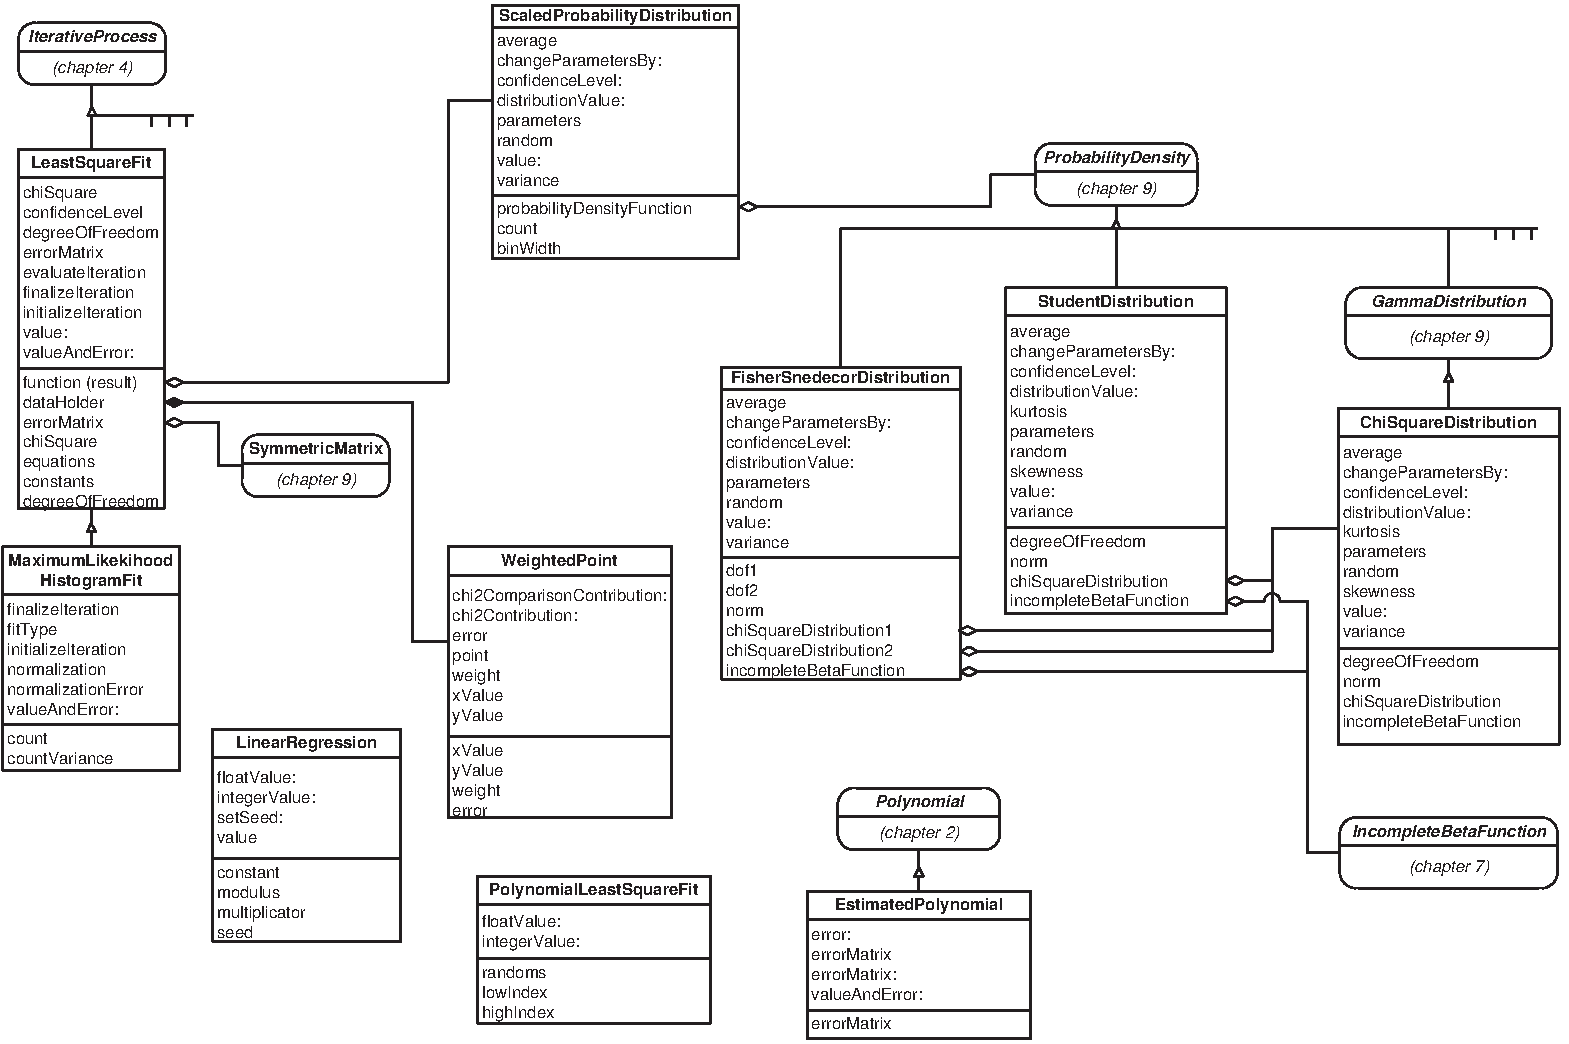
\includegraphics[width=11cm]{Figures/EstimationClasses}
\caption{Classes related to estimation}
\label{fig:estimationclasses}
\end{figure}
The reader should be aware that the techniques used for non-linear
least square fits (section \ref{sec:lsfnonlin}) can also be also
applied to solve systems of non-linear equations.

\section{$F$-test and the Fisher-Snedecor distribution}
\label{sec:Ftest} The $F$-test tries to answer the following
question: given two series of measurements, $x_1,\ldots,x_n$ and
$y_1,\ldots,y_m$, what is the probability that the two
measurements have the same standard deviation? The $F$-test is
used when there are not enough statistics to perform a detailed
analysis of the data.

Let us assume that the distribution of the two random variables,
$x$ and $y$, are normal distributions with respective averages
$\mu_x$ and $\mu_y$, and respective standard deviations $\sigma_x$
and $\sigma_y$. Then, $\bar{s}_x$, the standard deviation of
$x_1,\ldots,x_n$ is an estimator of $\sigma_x$; $\bar{s}_y$, the
standard deviation of $y_1,\ldots,y_m$ is an estimator of
$\sigma_y$. The following statistics
\begin{equation}
  F={\displaystyle \bar{s}_x^2\over\sigma_x^2}\cdot{\displaystyle\sigma_y^2\over\bar{s}_y^2}
\end{equation}
can be shown to be distributed according to a Fisher-Snedecor
distribution with degrees of freedom $n$ and $m$. In particular,
if one wants to test for the equality of the two standard
deviations, one construct the following statistics:
\begin{equation}
\label{eq:Ftest}
  F={\displaystyle \bar{s}_x^2\over\bar{s}_y^2}.
\end{equation}
Traditionally one chooses $\bar{s}_x>\bar{s}_y$ so that the
variable $F$ is always greater than one.

It is important to recall that the expression above is distributed
according to a Fisher-Snedecor distribution if and only if the two
sets of data are distributed according to a normal distribution.
For experimental measurements this is often the case unless
systematic errors are present. Nevertheless this assumption must
be verified before making an $F$-test.

Table \ref{tb:Fdist} shows the properties of the Fisher-Snedecor
distribution. The Fisher-Snedecor distribution is itself rarely
used as a probability density function, however.
\begin{table}[h]
  \centering
  \caption{Properties of the Fisher-Snedecor distribution}\label{tb:Fdist}
\vspace{1 ex}
\begin{tabular}{|l|c|} \hline
  \vbox to 3ex{}Range of random variable & $\left[0,+\infty\right[$\\ *[1ex] \hline
  \vbox to 5ex{}Probability density function & $\displaystyle P\left(x\right)=
  {n_1^{n_1\over 2}n_2^{n_2\over 2}x^{n_1-1\over 2}
  \over B\left({n_1\over 2},{n_2\over 2}\right)
  \left(n_1+n_2 x\right)^{n_1+n_2\over 2}
  }$ \\*[3ex]  \hline
  \vbox to 3ex{}Parameters & $n_1,n_2$ \\
  & two positive integers\\*[1ex]  \hline
  \vbox to 5ex{}Distribution function & $\displaystyle F\left(x\right)=
  B\left({n_1\over n_1+n_2x};{n_1\over 2},{n_2\over 2}\right)$ \\*[1ex]  \hline
  \vbox to 4ex{}Average & $\displaystyle{n_2\over n_2-2}$\quad for $n>2$ \\*[2ex]
  & undefined otherwise\\*[1ex] \hline
  \vbox to 5ex{}Variance & $\displaystyle{2n_2^2\left(n_1+n_2-2\right)\over
  n_1\left(n_2-2\right)^2\left(n_2-4\right)}$\quad for $n>4$ \\*[3ex]
  & undefined otherwise\\*[1ex] \hline
  \vbox to 3ex{}Skewness & $ $ \\*[1ex] \hline
  \vbox to 3ex{}Kurtosis & $ $ \\*[1ex] \hline
\end{tabular}
\end{table}

The main part of figure \ref{fig:fsnedecorDistr} shows the shape
of the Fisher-Snedecor distribution for some values of the degrees
of freedom.
\begin{figure}
\centering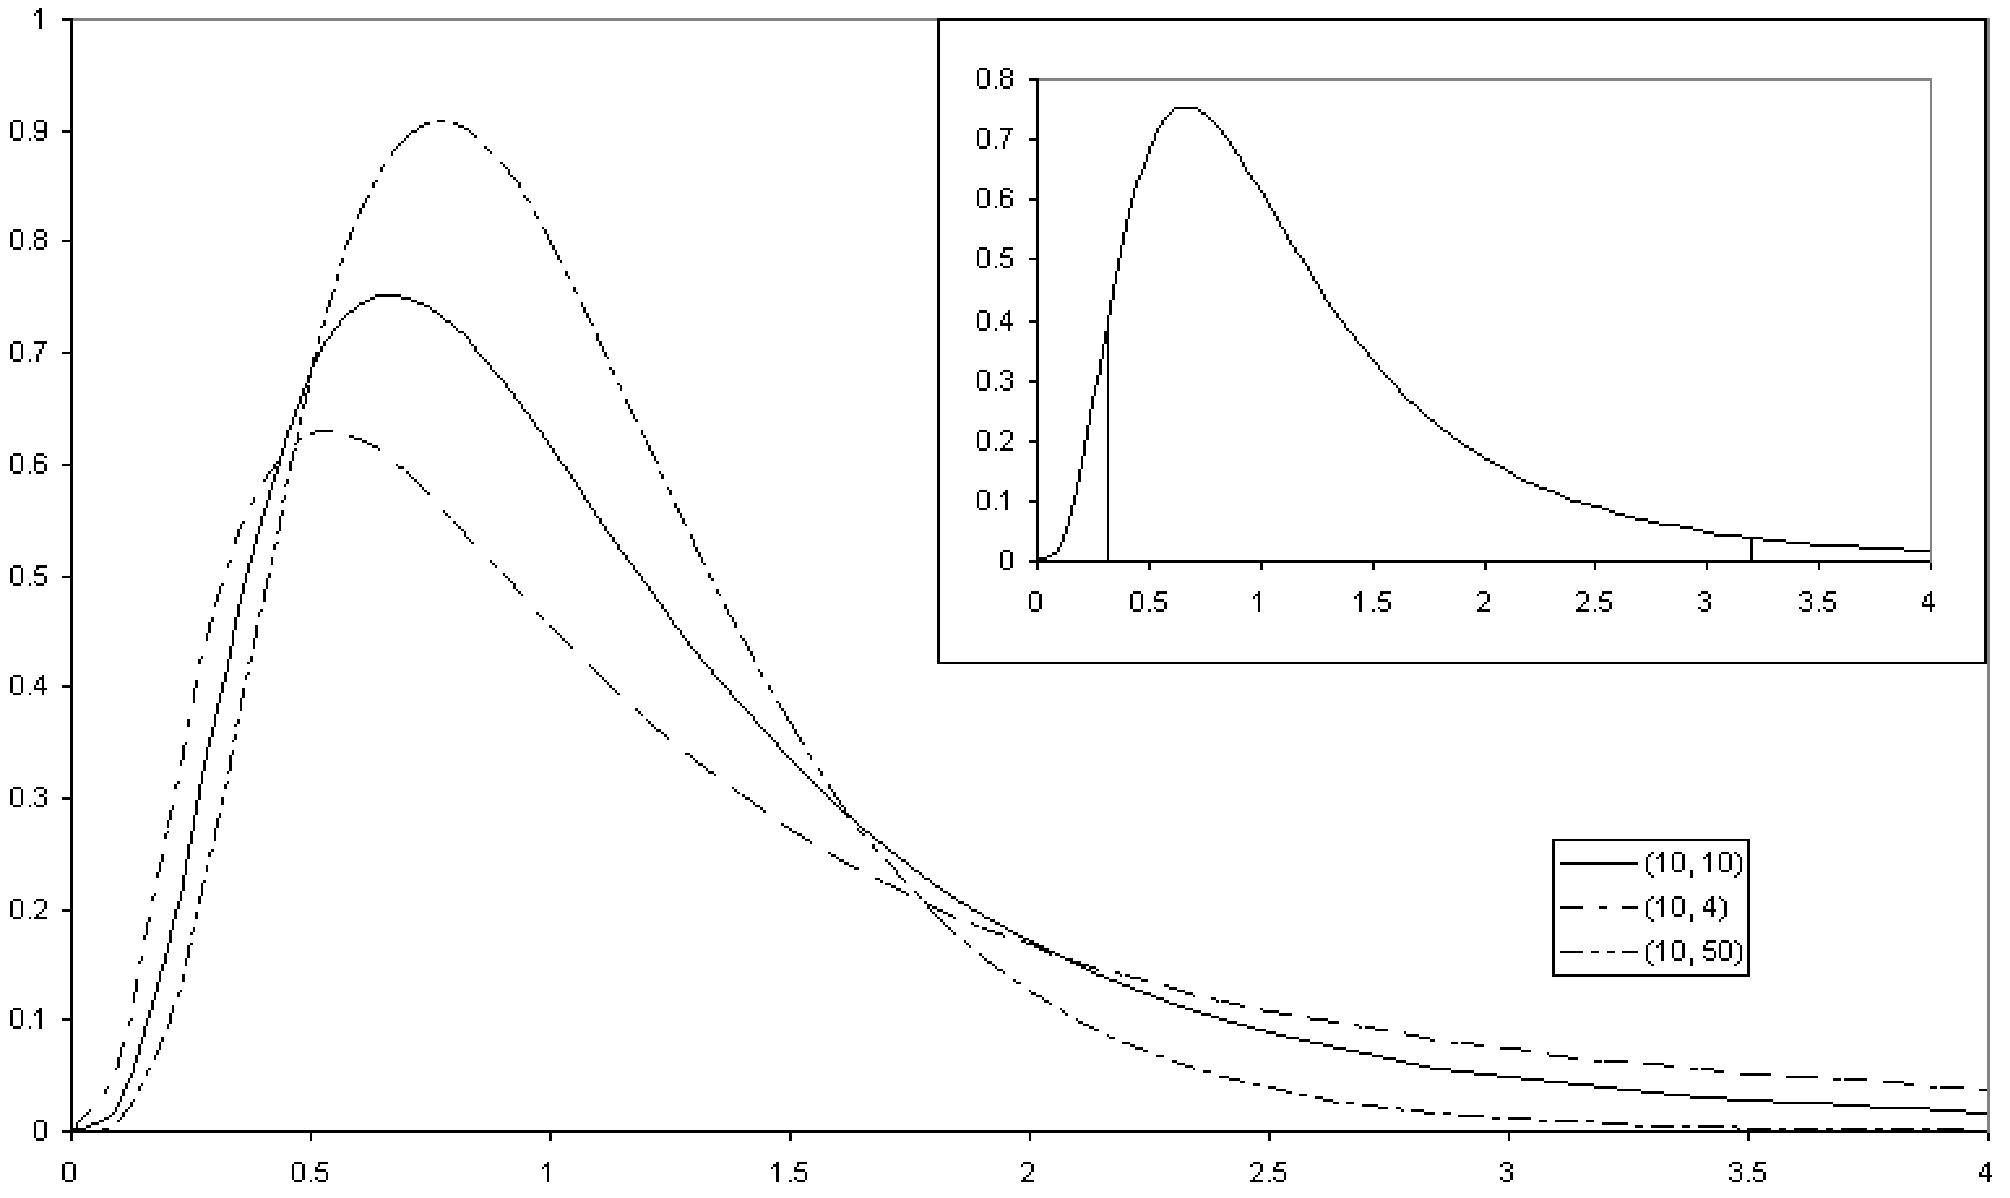
\includegraphics[width=12cm]{Figures/FisherSnedecorDistribution}
\caption{Fisher-Snedecor distribution for a few parameters}\label{fig:fsnedecorDistr}
\end{figure}
For large $n$ and $m$, the Fisher-Snedecor distribution
tends toward a normal distribution.


The confidence level of a Fisher-Snedecor distribution is defined
as the probability expressed in percent of finding a value larger
than $F$ defined in equation \ref{eq:Ftest} or lower than $1/F$.
The confidence level is thus related to the distribution function.
We have:
\begin{equation}
\label{eq:fcl}
  {\cl}_F\left(x,n\right)=100\left\{1-\left[F\left(x\right)-F\left({1\over x}\right)
  \right]\right\},
\end{equation}
where $x$ is the value $F$ defined in equation \ref{eq:Ftest}. The
change of notation was made to avoid confusion between the
acceptance function and the random variable.  The confidence level
corresponds to the surface of the shaded areas in the insert in
the upper right corner of figure \ref{fig:fsnedecorDistr}.

\rubrique{Example.} Here is an example used to investigate the
goodness of the two random number generators discussed in section
\ref{sec:random}. The collected data are the error of the
covariance test described in section \ref{sec:random}. The
dimension of the covariance matrix is 7 and the number of trials
on each measurement was 1000. The table \ref{tb:Ftest} presents
the obtained results, expressed in ${1\over 1000}$.
\begin{table}[h]
\vspace{1 ex}
  \centering
  \caption{Covariance test of random number generator}\label{tb:Ftest}
\vspace{1 ex}
  \begin{tabular}{|c|c|c|} \hline
     & Congruential & Mitchell-Moore \\ \hline
    1 & 5.56 & 7.48 \\
    2 & 5.89 & 6.75 \\
    3 & 4.66 & 3.77 \\
    4 & 5.69 & 5.71 \\
    5 & 5.34 & 7.25 \\
    6 & 4.79 & 4.73 \\
    7 & 4.80 & 6.23 \\
    8 & 7.86 & 5.60 \\
    9 & 3.64 & 5.94 \\
    10 & 5.70 & 4.58 \\ \hline
    Average & 5.40 & 5.80 \\
    Std. dev. & 1.10 & 1.19 \\ \hline
  \end{tabular}
\end{table}
the ratio of the two variances is $1.18$ and the degrees of
freedom are both 10. The F-test applied to the two variances gives
a confidence level of $20\%$. This means that there is only a
$20\%$ probability that the variances of the two series of
measurements are different.

\subsection{Fisher-Snedecor distribution --- Smalltalk implementation}
\marginpar{Figure \ref{fig:estimationclasses} with the box {\textbf
FisherSnedecorDistribution} grayed.} Listing \ref{ls:Fdist} shows
the implementation of the Fisher-Snedecor distribution in
Smalltalk. Listing \ref{ls:Ftest} shows the implementation of the
$F$-test in Smalltalk. The following code example shows how to
perform a $F$-test between two sets of experimental measurements.

\label{exs:Ftest}
\begin{displaycode}{Smalltalk}
 | mom1 mom2 confidenceLevel |
 mom1 := PMFixedStatisticalMoments new.
\end{displaycode}

\hfil{\texttt<\textsl Collecting measurements of set 1 into \texttt
mom1>}\hfil
\begin{displaycode}{Smalltalk}
 mom2 := PMFixedStatisticalMoments new.
\end{displaycode}
\hfil{\texttt<\textsl Collecting measurements of set 2 into \texttt
mom1>}\hfil
\begin{displaycode}{Smalltalk}
 confidenceLevel := mom1 fConfidenceLevel: mom2.
\end{displaycode}

Two instances of statistical moments (\cf section
\ref{sec:srobustmoment}) are created. Experimental data are
accumulated into each set separately (\cf code example
\ref{ex:smoments}). The last line returns the probability in
percent that the two sets of data have the same standard
deviation.

The class {\texttt PMFisherSnedecorDistribution} is implemented as a
subclass of {\texttt PMProbabilityDensity} because its distribution
function can be computed numerically using the incomplete beta
function (\cf section \ref{sec:incbeta}).

\begin{listing}[label=ls:Fdist]{Smalltalk}
{Smalltalk implementation of the Fisher-Snedecor distribution}
PMProbabilityDensity subclass: #PMFisherSnedecorDistribution
  instanceVariableNames: 'dof1 dof2 norm chiSquareDistribution1
  chiSquareDistribution2 incompleteBetaFunction'
  classVariableNames: ''
  package: 'Math-DistributionForHistogram'
\end{listing}

\begin{displaycode}{Smalltalk}
PMFisherSnedecorDistribution class >> degreeOfFreedom: anInteger1
degreeOfFreedom: anInteger2
    ^ super new initialize: anInteger1 and: anInteger2
\end{displaycode}

\begin{displaycode}{Smalltalk}
PMFisherSnedecorDistribution class >> distributionName
    ^ 'Fisher-Snedecor distribution'
\end{displaycode}

\begin{displaycode}{Smalltalk}
PMFisherSnedecorDistribution class >> fromHistogram: aHistogram
    | n1 n2 a |
    aHistogram minimum < 0 ifTrue: [^nil].
    n2 := (2 / (1 - (1 / aHistogram average))) rounded.
    n2 > 0 ifFalse: [^nil].
    a := (n2 - 2) * (n2 - 4) * aHistogram variance / (n2 squared * 
                                                                   2).
    n1 := (0.7 * (n2 - 2) / (1 - a)) rounded.
    ^n1 > 0 
        ifTrue: [self degreeOfFreedom: n1 degreeOfFreedom: n2]
        ifFalse: [nil]
\end{displaycode}

\begin{displaycode}{Smalltalk}
PMFisherSnedecorDistribution class >> new
 ^ self error: 'Illegal creation message for this class'
\end{displaycode} 

\begin{displaycode}{Smalltalk}
PMFisherSnedecorDistribution class >> test: aStatisticalMoment1 with: aStatisticalMoment2
    ^ (self class degreeOfFreedom: aStatisticalMoment1 count
        degreeOfFreedom: aStatisticalMoment2 count) 
            distributionValue: aStatisticalMoment1 variance 
                    / aStatisticalMoment2 variance
\end{displaycode}

\begin{displaycode}{Smalltalk}
PMFisherSnedecorDistribution >> average
    ^dof2 > 2
        ifTrue: [ dof2 / ( dof2 - 2) ]
        ifFalse:[ nil ]
\end{displaycode}
      
\begin{displaycode}{Smalltalk}
PMFisherSnedecorDistribution >> changeParametersBy: aVector
    dof1 := (dof1 + (aVector at: 1)) max: 1.
    dof2 := (dof2 + (aVector at: 2)) max: 1.
    self computeNorm.
    chiSquareDistribution1 := nil.
    chiSquareDistribution2 := nil.
    incompleteBetaFunction := nil
\end{displaycode}
  
\begin{displaycode}{Smalltalk}
PMFisherSnedecorDistribution >> computeNorm
    norm := (dof1 ln * (dof1 / 2)) + (dof2 ln * (dof2 / 2))
                        - ((dof1 / 2) logBeta: (dof2 / 2))
\end{displaycode}

\begin{displaycode}{Smalltalk}
PMFisherSnedecorDistribution >> confidenceLevel: aNumber
    aNumber < 0
        ifTrue: [ self error: 'Confidence level argument must be 
                                                           positive'].
    ^((self distributionValue: aNumber) - ( self distributionValue: 
                                           aNumber reciprocal) ) * 100
\end{displaycode}

\begin{displaycode}{Smalltalk}
PMFisherSnedecorDistribution >> distributionValue: aNumber
    ^ 1 - ( self incompleteBetaFunction value: ( dof2 / ( aNumber * 
                                                        dof1 + dof2)))
\end{displaycode}

\begin{displaycode}{Smalltalk}
PMFisherSnedecorDistribution >> incompleteBetaFunction
    incompleteBetaFunction isNil 
        ifTrue: 
            [incompleteBetaFunction := PMIncompleteBetaFunction 
                                                       shape: dof2 / 2
                        shape: dof1 / 2].
    ^incompleteBetaFunction
\end{displaycode}

\begin{displaycode}{Smalltalk}
PMFisherSnedecorDistribution >> initialize: anInteger1 and: anInteger2
    dof1 := anInteger1.
    dof2 := anInteger2.
    self computeNorm.
    ^ self
\end{displaycode}

\begin{displaycode}{Smalltalk}
PMFisherSnedecorDistribution >> parameters
    ^ Array with: dof1 with: dof2
\end{displaycode}

\begin{displaycode}{Smalltalk}
PMFisherSnedecorDistribution >> random
    chiSquareDistribution1 isNil
        ifTrue: [ chiSquareDistribution1 := PMChiSquareDistribution 
                                                degreeOfFreedom: dof1.
                  chiSquareDistribution2 := PMChiSquareDistribution 
                                                degreeOfFreedom: dof2.
                ].
    ^chiSquareDistribution1 random * dof2 / ( chiSquareDistribution2 
                                                        random * dof1)
\end{displaycode}

\begin{displaycode}{Smalltalk}
PMFisherSnedecorDistribution >> value: aNumber
    ^aNumber > 0
        ifTrue: [ (norm + ( aNumber ln * (dof1 / 2 - 1)) - ( 
             (aNumber * dof1 + dof2) ln * (( dof1 + dof2) / 2))) exp]
        ifFalse:[ 0 ]
\end{displaycode}

\begin{displaycode}{Smalltalk}
PMFisherSnedecorDistribution >> variance
    ^ dof2 > 4 ifTrue: [ dof2 squared * 2 * ( dof1 + dof2 - 2) / ( ( 
                              dof2 - 2) squared * dof1 * ( dof2 - 4))]
                   ifFalse:[ nil ]
\end{displaycode}

The computation of the confidence level for the $F$-test is
implemented in the method {\texttt fConfidenceLevel:} of the class
{\texttt PMStatisticalMoments}. It calculates the statistics $F$
according to equation \ref{eq:Ftest}, creates an instance of a
Fisher-Snedecor distribution and passes the value of $F$ to the
method {\texttt confidenceLevel:} of the distribution. The method {\texttt
fConfidenceLevel:} is also implemented by the class {\texttt
Histogram} where it is simply delegated to the statistical moments
accumulated by the histogram. The argument of the method can be a
statistical moment or a histogram since the messages sent by the
method are polymorphic to both classes.

\begin{listing} Smalltalk implementation of the $F$-test \label{ls:Ftest}
$$\halign{ #\hfil&\quad#\hfil\cr {\sl Class}& {\Large\bf DhbStatisticalMoments}\cr
{\sl Subclass of }&{\tt Object}\cr\noalign{\vskip 1ex}

{\sl Instance variable names:}&\parbox[t]{4 in}{\tt  moments }\cr\noalign{\vskip 1ex}}$$


Instance methods
{\parskip 1ex\par\noindent}
{\bf fConfidenceLevel:} {\tt aStatisticalMomentsOrHistogram}
\begin{verbatim}
    | fValue |
    fValue := self variance/ aStatisticalMomentsOrHistogram variance.
    ^ fValue < 1
        ifTrue: [ (DhbFisherSnedecorDistribution degreeOfFreedom: 
                                  aStatisticalMomentsOrHistogram count
                        degreeOfFreedom: self count) 
                                        confidenceLevel: fValue 
                                                           reciprocal ]
        ifFalse: [ (DhbFisherSnedecorDistribution degreeOfFreedom: 
                                                            self count
                        degreeOfFreedom: 
                                aStatisticalMomentsOrHistogram count) 
                                        confidenceLevel: fValue ]
\end{verbatim}


$$\halign{ #\hfil&\quad#\hfil\cr {\sl Class}& {\Large\bf DhbHistogram}\cr
{\sl Subclass of }&{\tt Object}\cr\noalign{\vskip 1ex}

{\sl Instance variable names:}&\parbox[t]{4 in}{\tt  minimum binWidth overflow underflow moments contents freeExtent cacheSize desiredNumberOfBins }\cr\noalign{\vskip 1ex}}$$

Instance methods
{\parskip 1ex\par\noindent}
{\bf fConfidenceLevel:} {\tt aStatisticalMomentsOrHistogram}
\begin{verbatim}
    ^ moments fConfidenceLevel: aStatisticalMomentsOrHistogram
\end{verbatim}


\end{listing}

\section{$t$-test and the Student distribution}
\label{sec:ttest} The $t$-test tries to answer the following
question: given two series of measurements, $x_1,\ldots,x_n$ and
$y_1,\ldots,y_m$, what is the probability that the two
measurements have the same average?  The $t$-test is used when
there are not enough statistics to perform a detailed analysis of
the data.

Let us assume that the distribution of the two random variables,
$x$ and $y$, are normal distributions with respective averages
$\mu_x$ and $\mu_y$, and the same standard deviation $\sigma$.
Then $\bar{x}$, the average of $x_1,\ldots,x_n$ is an estimator of
$\mu_x$; $\bar{y}$, the average of $y_1,\ldots,y_m$ is an
estimator of $\mu_y$. An estimation $\bar{s}$ of the standard
deviation $\sigma$ can be made using both measurement samples. We
have:
\begin{equation}
\label{eq:sbart}
  \bar{s}^2={\displaystyle\sum_{i=1}^n\left(x_i-\bar{x}\right)^2
  + \sum_{i=1}^m\left(y_i-\bar{y}\right)^2\over\displaystyle n+m-2}.
\end{equation}
One can prove that the following statistics:
\begin{equation}
  t={\displaystyle \left(\bar{x}-\bar{y}\right)-\left(\mu_x
  -\mu_y\right)
  \over\displaystyle \bar{s}\sqrt{{1\over n}+{1\over m}}}
\end{equation}
is distributed according to a Student distribution with $n+m-2$
degrees of freedom. In particular, to test for the probability
that the two series of measurements have the same average, one
uses the following statistics:
\begin{equation}
\label{eq:tTest}
  t={\displaystyle \bar{x}-\bar{y}
  \over\displaystyle \bar{s}\sqrt{{1\over n}+{1\over m}}}.
\end{equation}
It is important to recall the two fundamental hypotheses that have
been made so far.
\begin{enumerate}
  \item The two sets of data must be distributed according to a normal distribution.
  \item The two sets of data must have the same standard deviation.
\end{enumerate}
Too many people use the $t$-test without first checking the
assumptions. Assumption 1 is usually fulfilled with experimental
measurements in the absence of systematic errors. Assumption 2.
however, must be checked, for example using the F-test discussed
in section \ref{sec:Ftest}.

Because the random variable of the distribution is traditionally
labeled $t$, this distribution is often called the
$t$-distribution. Table \ref{tb:tdist} shows the properties of the
Student distribution. The Student distribution is itself rarely
used as a probability density function, however.
\begin{table}[h]
  \centering
  \caption{Properties of the Student distribution}\label{tb:tdist}
\vspace{1 ex}
\begin{tabular}{|l|c|} \hline
  \vbox to 3ex{}Range of random variable & $\left]-\infty,+\infty\right[$\\ *[1ex] \hline
  \vbox to 5ex{}Probability density function & $\displaystyle P\left(x\right)=
  {1\over\sqrt{n}B\left({n\over 2},{1\over 2}\right)}
  \left(1+{t^2\over n}\right)^{-{n+1\over 2}}$ \\*[2ex]  \hline
  \vbox to 3ex{}Parameters & $n$ \\
  & a positive integer\\*[1ex]  \hline
  \vbox to 4ex{}Distribution function &
  \parbox{6cm}{$$F\left(x\right)=\left\{
  \begin{array}{ll}
  {1 + B\left({n\over n + x^2};{n\over 2},{1\over 2}\right)\over 2}&\mbox{\quad for
  $x\ge 0$}\\*[1ex]
  {1 - B\left({n\over n + x^2};{n\over 2},{1\over 2}\right)\over 2}&\mbox{\quad for $x<0$}
  \end{array}\right.$$} \\*[1ex]  \hline
  \vbox to 3ex{}Average & $0$ \\*[1ex] \hline
  \vbox to 3ex{}Variance & ${n\over n-2}$\quad for $n>2$\\
  & undefined otherwise\\*[1ex] \hline
  \vbox to 3ex{}Skewness & $0$ \\*[1ex] \hline
  \vbox to 3ex{}Kurtosis & ${6\over n-4}$\quad for $n>4$\\
  & undefined otherwise\\*[1ex] \hline
\end{tabular}
\end{table}

For $n=1$, the Student distribution is identical to a Cauchy
distribution with $\mu=0$ and $\beta=1$. For large $n$, the
Student distribution tends toward a normal distribution with
average 0 and variance 1. The main part of figure
\ref{fig:studentDistr} shows the shapes of the Student
distribution for a few values of the degrees of freedom. The
normal distribution is also given for comparison.
\begin{figure}
\centering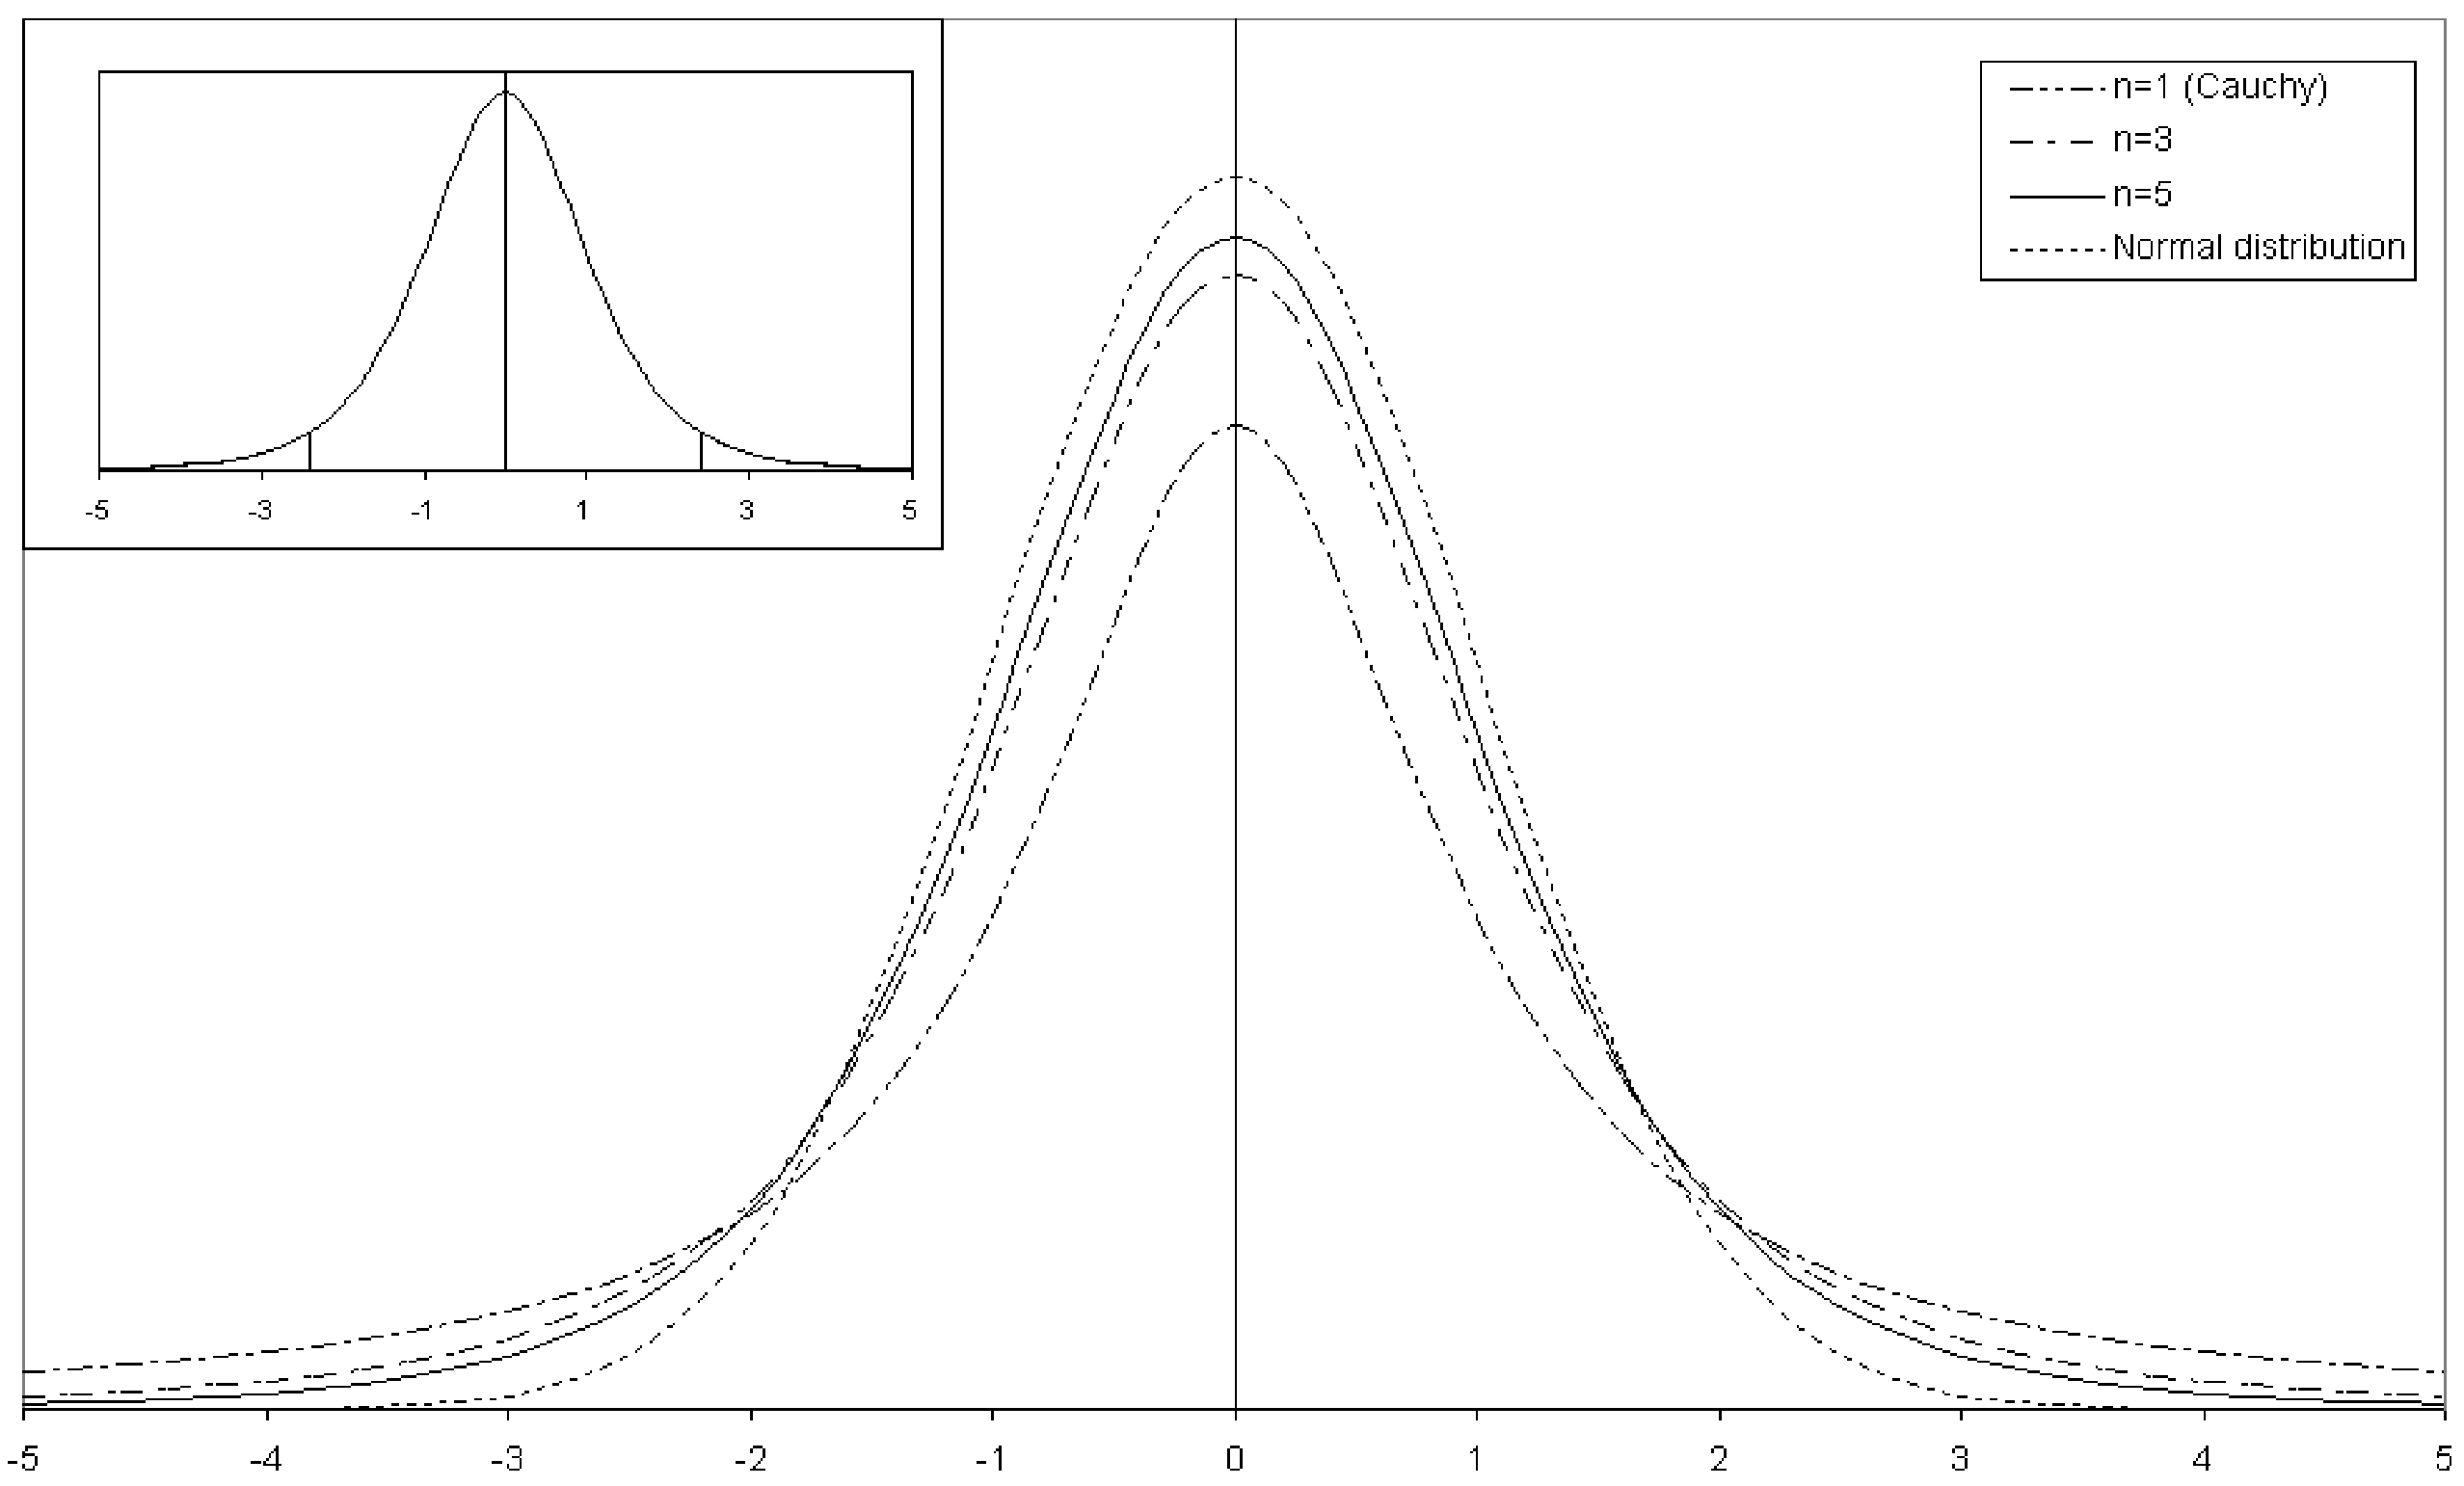
\includegraphics[width=12cm]{Figures/StudentDistribution}
\caption{Student distribution for a few degrees of freedom
}\label{fig:studentDistr}
\end{figure}


The confidence level of a Student distribution is defined as the
probability to find a value whose absolute value is larger than a
given value. Thus, it estimates the level of confidence that the
hypothesis --- namely, that the two sets of measurements have the
same average --- cannot be accepted. Traditionally the confidence
level is given in percent. The confidence level corresponds to the
surface of shaded area in the insert in the upper left corner of
figure \ref{fig:studentDistr}. By definition, the confidence level
is related to the interval acceptance function:
\begin{equation}
\label{eq:tcl}
  {\cl}_t\left(t,n\right)=100\left[1-
  F\left(-\left|t\right|,\left|t\right|\right)\right],
\end{equation}
using the definition of the interval acceptance function (equation
\ref{eq:defacceptdiff}). The value of $t$ in equation \ref{eq:tcl}
is obtained from equation \ref{eq:tTest}.

The distribution function of the Student distribution is
calculated with the incomplete beta function (\cf section
\ref{sec:incbeta}). Using the fact that the distribution is
symmetric, one can derive the following expression
\begin{equation}
\label{eq:tsymacc}
  F\left(-\left|t\right|,\left|t\right|\right)=B\left({n\over n + t^2};{n\over 2},{1\over
  2}\right),
\end{equation}
from the properties of the distribution (\cf table \ref{tb:tdist})
and using equations \ref{eq:tcl} and \ref{eq:incBetaFunction}.

\rubrique{Example} Now, we shall continue the analysis of the
results of table \ref{tb:Ftest}. The $t$ value computed from the
two sets of measurements is $0.112$ for a degree of freedom of 18.
the corresponding confidence level is $8.76\%$. That is, there is
only a $8.76\%$ probability that the two generators have a
different behavior. Thus, we can conclude that the Mitchell-Moore
random generator is as good as the congruential random generator.

\subsection{Student distribution --- Smalltalk implementation}
\marginpar{Figure \ref{fig:estimationclasses} with the box {\textbf
StudentDistribution} grayed.} Listing \ref{ls:tdist} shows the
implementation of the Student distribution in Smalltalk. Listing
\ref{ls:tTest} shows the implementation of the $t$-test in
Smalltalk. Performing a $t$-test between two sets of experimental
measurements is very similar to performing a $F$-test. In code
example \ref{exs:Ftest} it suffices to replace the last line with
the following:
\begin{displaycode}
 confidenceLevel := mom1 fConfidenceLevel: mom2.
\end{displaycode}
This last line returns the probability in percent that the two
sets of data have the same average provided that the two sets have
the same standard deviation.

The class {\texttt PMStudentDistribution} is implemented as a
subclass of {\texttt PMProbabilityDensity} because its distribution
function can be computed numerically using the incomplete beta
function (\cf section \ref{sec:incbeta}).

The method {\texttt symmetricAcceptance:} computes the symmetric
acceptance function defined by equation \ref{eq:tsymacc}. This
method is used to compute the disribution function and the
confidence level. The method {\texttt confidenceLevel:} gives the
confidence level in percent.
\begin{listing} Smalltalk implementation of the Student distribution \label{ls:tdist}
$$\halign{ #\hfil&\quad#\hfil\cr {\sl Class}& {\Large\bf DhbStudentDistribution}\cr
{\sl Subclass of }&{\tt DhbProbabilityDensity}\cr\noalign{\vskip 1ex}

{\sl Instance variable names:}&\parbox[t]{4 in}{\tt  degreeOfFreedom norm chiSquareDistribution incompleteBetaFunction }\cr\noalign{\vskip 1ex}}$$


Class methods
{\parskip 1ex\par\noindent}
{\bf asymptoticLimit}
\begin{verbatim}
    ^ 30
\end{verbatim}
{\bf degreeOfFreedom:} {\tt anInteger}
\begin{verbatim}
    ^anInteger > self asymptoticLimit 
        ifTrue: [DhbNormalDistribution new]
        ifFalse: 
            [anInteger = 1 
                ifTrue: [DhbCauchyDistribution shape: 0 scale: 1]
                ifFalse: [super new initialize: anInteger]]
\end{verbatim}
{\bf distributionName}
\begin{verbatim}
    ^'Student distribution'
\end{verbatim}
{\bf fromHistogram:} {\tt aHistogram}
\begin{verbatim}
    | dof var |
    var := aHistogram variance.
    var = 0
        ifTrue: [ ^nil].
    dof :=  ( 2 / (1 - (1 / aHistogram variance))) rounded max: 1.
    ^dof > self asymptoticLimit ifTrue: [ nil]
                                ifFalse:[ self degreeOfFreedom: dof]
\end{verbatim}
{\bf new}
\begin{verbatim}
    ^self error: 'Illegal creation message for this class'
\end{verbatim}
{\bf test:} {\tt aStatisticalMoment1} {\bf with:} {\tt aStatisticalMoment2}
\begin{verbatim}
    | t |
    t := ( aStatisticalMoment1 average - aStatisticalMoment2 average) 
                                                                  abs.
    ^1 - ( ( self class degreeOfFreedom: (  aStatisticalMoment1 count 
  + aStatisticalMoment2 count - 2)) acceptanceBetween: t negated and: 
  t)
\end{verbatim}



Instance methods
{\parskip 1ex\par\noindent}
{\bf average}
\begin{verbatim}
    ^ 0
\end{verbatim}
{\bf changeParametersBy:} {\tt aVector}
\begin{verbatim}
    degreeOfFreedom := degreeOfFreedom + ( aVector at: 1).
    self computeNorm.
\end{verbatim}
{\bf chiSquareDistribution}
\begin{verbatim}
    chiSquareDistribution isNil
        ifTrue: [ chiSquareDistribution := DhbChiSquareDistribution 
                              degreeOfFreedom: (degreeOfFreedom - 1)].
    ^ chiSquareDistribution
\end{verbatim}
{\bf computeNorm}
\begin{verbatim}
    norm := ( ( degreeOfFreedom / 2 logBeta: ( 1 / 2) ) + ( 
                                     degreeOfFreedom ln / 2)) negated.
\end{verbatim}
{\bf confidenceLevel:} {\tt aNumber}
\begin{verbatim}
    ^ (1 - (self symmetricAcceptance: aNumber abs)) * 100
\end{verbatim}
{\bf distributionValue:} {\tt aNumber}
\begin{verbatim}
    aNumber = 0
        ifTrue: [ ^0.5].
    ^ (aNumber > 0
        ifTrue: [ 2 - (self symmetricAcceptance: aNumber abs) ]
        ifFalse:[ self symmetricAcceptance: aNumber abs ]) / 2

\end{verbatim}
{\bf incompleteBetaFunction}
\begin{verbatim}
    incompleteBetaFunction isNil 
        ifTrue: 
            [incompleteBetaFunction := DhbIncompleteBetaFunction 
                        shape: degreeOfFreedom / 2
                        shape: 0.5].
    ^ incompleteBetaFunction
\end{verbatim}
{\bf initialize:} {\tt anInteger}
\begin{verbatim}
    anInteger > 0
        ifFalse: [ self error: 'Degree of freedom must be positive'].
    degreeOfFreedom := anInteger.
    self computeNorm.
    ^ self
\end{verbatim}
{\bf kurtosis}
\begin{verbatim}
    ^ degreeOfFreedom > 4 ifTrue: [ 6 / ( degreeOfFreedom - 4)]
                         ifFalse: [ nil ]
\end{verbatim}
{\bf parameters}
\begin{verbatim}
    ^Array with: degreeOfFreedom
\end{verbatim}
{\bf random}
\begin{verbatim}
    ^DhbNormalDistribution random * ( ( (degreeOfFreedom - 1) / self 
                                  chiSquareDistribution random ) sqrt)
\end{verbatim}
{\bf skewness}
\begin{verbatim}
    ^ 0
\end{verbatim}
{\bf symmetricAcceptance:} {\tt aNumber}
\begin{verbatim}
    ^ self incompleteBetaFunction value: ( degreeOfFreedom / ( 
                                   aNumber squared + degreeOfFreedom))
\end{verbatim}
{\bf value:} {\tt aNumber}
\begin{verbatim}
    ^(norm - ((aNumber squared / degreeOfFreedom + 1) ln * ( ( 
                                       degreeOfFreedom + 1) / 2))) exp
\end{verbatim}
{\bf variance}
\begin{verbatim}
    ^ degreeOfFreedom > 2 ifTrue: [ degreeOfFreedom / ( 
                                                 degreeOfFreedom - 2) ]
                         ifFalse:[ nil ]
\end{verbatim}


\end{listing}

The computation of the confidence level for the $t$-test is
implemented in the method {\texttt tConfidenceLevel:} of the class
{\texttt PMStatisticalMoments}. It calculates the statistics $t$
according to equation \ref{eq:tTest}, creates an instance of a
Student distribution and passes the value of $t$ to the method
{\texttt confidenceLevel:} of the distribution. The method {\texttt
tConfidenceLevel:} is also implemented by the class {\texttt
Histogram} where it is simply delegated to the statistical moments
accumulated by the histogram. The argument of the method can be a
statistical moment or a histogram since the messages sent by the
method are polymorphic to both classes.

The method {\texttt unnormalizedVariance} of class {\texttt
PMStatisticalMoments} corresponds to each sums in the numerator
of equation \ref{eq:sbart}. To allow performing a $t$-test also
with instances of class {\texttt PMFastStatisticalMoments}, it was
necessary to define this for that class.

\begin{listing} Smalltalk implementation of the $t$-test \label{ls:tTest}
$$\halign{ #\hfil&\quad#\hfil\cr {\sl Class}& {\Large\bf DhbStatisticalMoments}\cr
{\sl Subclass of }&{\tt Object}\cr\noalign{\vskip 1ex}

{\sl Instance variable names:}&\parbox[t]{4 in}{\tt  moments }\cr\noalign{\vskip 1ex}}$$


Instance methods
{\parskip 1ex\par\noindent}
{\bf tConfidenceLevel:} {\tt aStatisticalMomentsOrHistogram}
\begin{verbatim}
    | sbar dof |
    dof := self count + aStatisticalMomentsOrHistogram count - 2.
    sbar := ( ( self unnormalizedVariance + 
     aStatisticalMomentsOrHistogram unnormalizedVariance) / dof) sqrt.
    ^( DhbStudentDistribution degreeOfFreedom: dof)
        confidenceLevel: ( self average - 
                             (aStatisticalMomentsOrHistogram average))
                            / ( ( 1 / self count + ( 
                   aStatisticalMomentsOrHistogram count)) sqrt * sbar)

\end{verbatim}


$$\halign{ #\hfil&\quad#\hfil\cr {\sl Class}& {\Large\bf DhbFastStatisticalMoments}\cr
{\sl Subclass of }&{\tt DhbStatisticalMoments}\cr\noalign{\vskip 1ex}
}$$


Instance methods
{\parskip 1ex\par\noindent}
{\bf unnormalizedVariance}
\begin{verbatim}
    ^ (moments at: 3) - ((moments at: 2) squared * self count)
\end{verbatim}


$$\halign{ #\hfil&\quad#\hfil\cr {\sl Class}& {\Large\bf DhbHistogram}\cr
{\sl Subclass of }&{\tt Object}\cr\noalign{\vskip 1ex}

{\sl Instance variable names:}&\parbox[t]{4 in}{\tt  minimum binWidth overflow underflow moments contents freeExtent cacheSize desiredNumberOfBins }\cr\noalign{\vskip 1ex}}$$


Instance methods
{\parskip 1ex\par\noindent}
{\bf tConfidenceLevel:} {\tt aStatisticalMomentsOrHistogram}
\begin{verbatim}
    ^moments tConfidenceLevel: aStatisticalMomentsOrHistogram

\end{verbatim}
{\bf unnormalizedVariance}
\begin{verbatim}
    ^moments unnormalizedVariance

\end{verbatim}


\end{listing}

\section{$\chi^2$-test and $\chi^2$ distribution}
\label{sec:chitest} The $\chi^2$-test tries to answer the
following question: how well a theory is able to predict observed
results? Alternatively a $\chi^2$-test can also tell whether two
independent sets of observed results are compatible. This latter
formulation is less frequently used than the former. Admittedly
these two questions are somewhat vague. We shall now put them in
mathematical terms for a more precise definition.

Let us assume that the measurement of an observable quantity
depends on some parameters. These parameters cannot be adjusted by
the experimenter but can be measured exactly\footnote{Of course,
there is no such thing as an exact measurement. The measurement of
the parameters must be far more precise than that of the observed
quantity.}. Let $x_p$ be the measured values of the observed
quantity where $p$ is a label for the parameters; let $\sigma_p$
be the standard deviation of $x_p$.

The first question assumes that one can predict the values of the
observed quantity: let $\mu_p$ be the predicted value of $x_p$.
Then the quantity:
\begin{equation}
  y_p = { x_p - \mu_p \over \sigma_p}
\end{equation}
is distributed according to a normal distribution with average 0
and standard deviation 1 if and only if the quantities $x_p$ are
distributed according to a normal distribution with average
$\mu_p$ and standard deviation $\sigma_p$.

A $\chi^2$ distribution with $n$ degrees of freedom describes the
distribution of the sum of the squares of $n$ random variables
distributed according to a normal distribution with mean 0 and
standard deviation 1. Thus, the following quantity
\begin{equation}
\label{eq:defchitest}
  S=\sum_p { \left(x_p - \mu_p\right)^2\over \sigma_p^2}
\end{equation}
is distributed according to a $\chi^2$ distribution with $n$
degrees of freedom where $n$ is the number of available
measurements (that is the number of terms in the sum of equation
\ref{eq:defchitest}).

To formulate the second question one must introduce a second set
of measurement of the same quantity and at the same values of the
parameters. Let $x^{\prime}_p$ be the second set of measured
values and $\sigma^{\prime}_p$ the corresponding standard
deviations. The estimated standard deviation for the difference
$x_p - x^{\prime}_p$ is $\sqrt{\sigma_p^2+\sigma^{\prime 2}_p }$.
If the two sets of measurements are compatible, the quantity
\begin{equation}
  y^{\prime}_p = { x_p - x^{\prime}_p \over
  \sqrt{\sigma_p^2+\sigma^{\prime 2}_p}}
\end{equation}
is distributed according to a normal distribution with average 0
and standard deviation 1. Then the following quantity
\begin{equation}
\label{eq:defchitestcmp}
  S=\sum_p { \left(x_p - x^{\prime}_p\right)^2\over \sigma_p^2+\sigma^{\prime 2}_p2}
\end{equation}
is distributed according to a $\chi^2$ distribution with $n$
degrees of freedom.

Table \ref{tb:chi2dist} shows the properties of the $\chi^2$
distribution.
\begin{table}[h]
  \centering
  \caption{Properties of the $\chi^2$ distribution}\label{tb:chi2dist}
\vspace{1 ex}
\begin{tabular}{|l|c|} \hline
  \vbox to 3ex{}Range of random variable & $\left[0,+\infty\right[$\\ *[1ex] \hline
  \vbox to 5ex{}Probability density function & $\displaystyle P\left(x\right)=
  {\displaystyle x^{{n\over 2}-1}e^{-{x\over 2}}
  \over\displaystyle 2^{n\over 2}\Gamma\left({n\over 2}\right)}$ \\*[4ex]  \hline
  \vbox to 3ex{}Parameters & $n$ \\
  & a positive integer\\*[1ex]  \hline
  \vbox to 4ex{}Distribution function & $\displaystyle F\left(x\right)=
  \Gamma\left({x\over 2};{n\over 2}\right)$ \\*[1ex]  \hline
  \vbox to 3ex{}Average & $n$ \\*[1ex] \hline
  \vbox to 3ex{}Variance & $2n$ \\*[1ex] \hline
  \vbox to 4ex{}Skewness & $2\sqrt{\displaystyle 2\over\displaystyle n}$ \\*[1ex] \hline
  \vbox to 4ex{}Kurtosis & ${\displaystyle 12\over\displaystyle n}$ \\*[1ex] \hline
\end{tabular}
\end{table}
It is a special case of the gamma distribution with
$\alpha={n\over 2}$ and $\beta=2$ (\cf section
\ref{sec:gammadist}). For $n>30$ one can prove that the variable
$y=\sqrt{2x}-\sqrt{2n-1}$ is approximately distributed according
to a normal distribution with average 0 and standard deviation 1.
If $n$ is very large the $\chi^2$ distribution tends toward a
normal distribution with average $n$ and standard deviation
$\sqrt{2n}$.

Figure \ref{fig:chi2Distr} shows the shape of the $\chi^2$
distribution for a few values of the degree of freedom.
\begin{figure}
\centering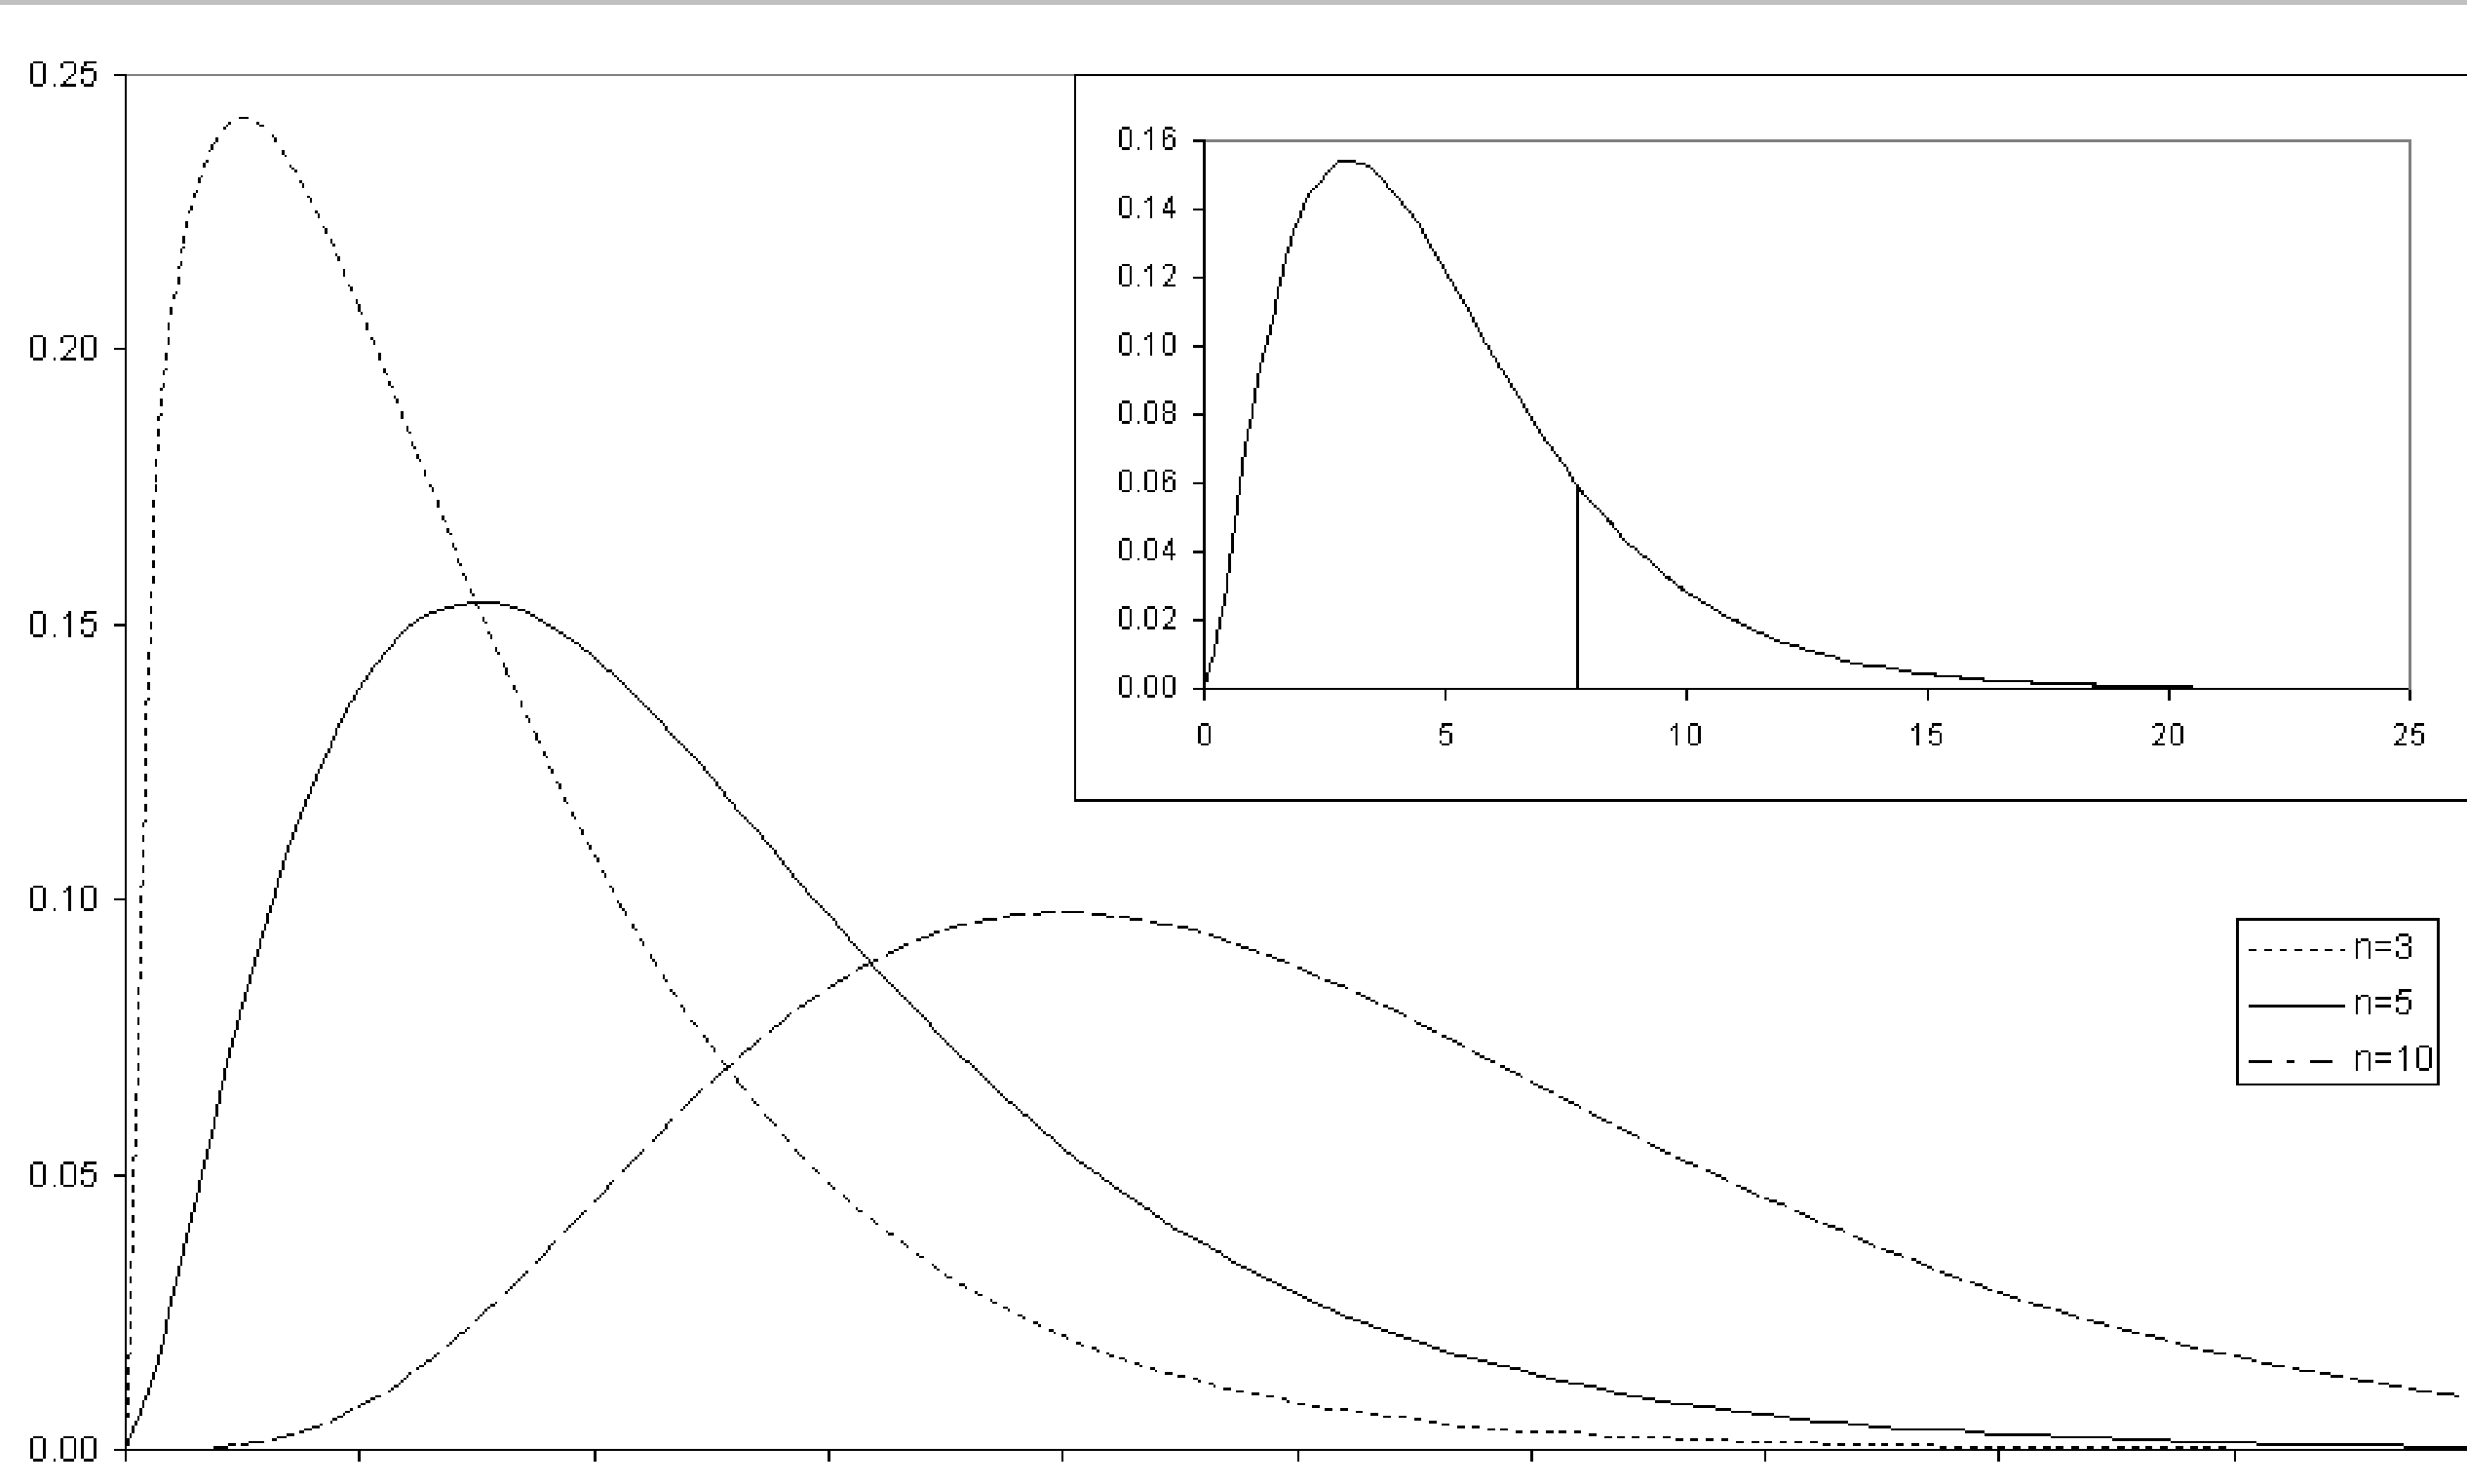
\includegraphics[width=12cm]{Figures/Chi2Distribution}
\caption{$\chi^2$ distribution for a few degrees of freedom
}\label{fig:chi2Distr}
\end{figure}


To perform a $\chi^2$-test, it is customary to evaluate the
probability of finding a value larger than the value obtained in
equations \ref{eq:defchitest} or \ref{eq:defchitestcmp}. In this
form, the result of a $\chi^2$-test gives the probability that the
set of measurements is {\textsl not} compatible with the prediction or
with another set of measurements. The confidence level of a
$\chi^2$ value is defined as the probability of finding a value
larger than $\chi^2$ expressed in percent. It is thus related to
the distribution function as follows:
\begin{equation}
  {\cl}_{S}=100\left[ 1-F\left(S\right)\right],
\end{equation}
where $S$ is the quantity defined in equation \ref{eq:defchitest}
or \ref{eq:defchitestcmp}. The confidence level corresponds to the
surface of the shaded area of the insert in the upper right corner
of figure \ref{fig:chi2Distr}.

Since the $\chi^2$ distribution is a special case of the gamma
distribution the confidence level can be expressed with the
incomplete gamma function (\cf section \ref{sec:incGamma}):
\begin{equation}
\label{eq:chiTest}
  {\cl}_{S}=100\left[ 1-\Gamma\left({S \over 2},{n\over 2}\right)\right].
\end{equation}
For large $n$ the $\chi^2$ confidence level can be computed from
the error function (\cf section \ref{sec:errorFunctionDef}):
\begin{equation}
\label{eq:chiTestAsymp}
  {\cl}_{S}=100\left[ 1-\erf\left(\sqrt{2S}-\sqrt{2n-1}\right)\right].
\end{equation}

\subsection{$\chi^2$ distribution --- Smalltalk implementation}
\marginpar{Figure \ref{fig:estimationclasses} with the box {\textbf
ChiSquaredDistribution} grayed.} Listing \ref{ls:chidist} shows
the implementation of the $\chi^2$ distribution in Smalltalk. The
asymptotic limit is implemented directly in the class creation
method.
\begin{listing} Smalltalk implementation of the $\chi^2$ distribution \label{ls:chidist}
$$\halign{ #\hfil&\quad#\hfil\cr {\sl Class}& {\Large\bf DhbChiSquareDistribution}\cr
{\sl Subclass of }&{\tt DhbGammaDistribution}\cr\noalign{\vskip 1ex}
}$$


Class methods
{\parskip 1ex\par\noindent}
{\bf degreeOfFreedom:} {\tt anInteger}
\begin{verbatim}
    ^anInteger > 40
        ifTrue: [ DhbAsymptoticChiSquareDistribution degreeOfFreedom: 
                                                            anInteger]
        ifFalse:[ super shape: anInteger / 2 scale: 2]

\end{verbatim}
{\bf distributionName}
\begin{verbatim}
    ^'Chi square distribution'
\end{verbatim}
{\bf fromHistogram:} {\tt aHistogram}
\begin{verbatim}
    | dof |
    aHistogram minimum < 0
        ifTrue: [ ^nil].
    dof := aHistogram average rounded.
    ^dof > 0 ifTrue: [ self degreeOfFreedom: aHistogram average 
                                                              rounded]
             ifFalse:[ nil ]
\end{verbatim}
{\bf shape:} {\tt aNumber1} {\bf scale:} {\tt aNumber2}
\begin{verbatim}
    ^self error: 'Illegal creation message for this class'
\end{verbatim}



Instance methods
{\parskip 1ex\par\noindent}
{\bf changeParametersBy:} {\tt aVector}
\begin{verbatim}
    super changeParametersBy: (Array with: aVector first / 2 with: 0).
\end{verbatim}
{\bf confidenceLevel:} {\tt aNumber}
\begin{verbatim}
    ^ (1 - ( self distributionValue: aNumber)) *100
\end{verbatim}
{\bf parameters}
\begin{verbatim}
    ^ Array with: alpha * 2
\end{verbatim}


\end{listing}


\subsection{Weighted point implementation}
\label{sec:weightedPoint} \marginpar{Figure
\ref{fig:estimationclasses} with the box {\textbf WeightedPoint}
grayed.} As we shall see in the rest of this chapter, the
evaluation of equation \ref{eq:defchitest} is performed at many
places. Thus, it is convenient to create a new class handling this
type of calculation.
The new class is called {\texttt PMWeightedPoint} in Smalltalk.

\noindent A weighted point has the following instance variables:
\begin{description}
  \item[\texttt xValue] the $x$ value of the data point, that is $x_i$,
  \item[\texttt yValue] the $y$ value of the data point, that is $y_i$,
  \item[\texttt weight] the weight of the point, that is $1/\sigma_i^2$
  and
  \item[\texttt error] the error of the $y$ value, that is $\sigma_i$.
\end{description}
Accessor methods for each of these instance variables are
provided. The accessor method for the error is using lazy
initialization to compute the error from the weight in case the
error has not yet been defined.

The method {\texttt chi2Contribution} --- with an added semicolon at
the end of the name for Smalltalk --- implements the computation
of one term of the sum in equation \ref{eq:defchitest}. The
argument of the method is any object implementing the behavior of
a one-variable function defined in section \ref{sec:function}.

Creating instances of the classes can be done in many ways. The
fundamental method takes as arguments $x_i$, $y_i$ and the weight
$1/\sigma_i^2$. However convenience methods are provided for
frequent cases:
\begin{enumerate}
  \item $x_i$, $y_i$ and the error on $y_i$, $\sigma_i$;
  \item $x_i$ and the content of a histogram bin; the weight is derived
  from the bin contents as explained in section \ref{sec:chitesthist};
  \item $x_i$, $y_i$ without known error; the weight of the point is set to
  1; points without error should not be used together with points
  with errors;
  \item $x_i$ and a statistical moment; in this case, the value $y_i$
  is an average over a set of measurements; the weight is determined
  from the error on the average (\cf section \ref{sec:moments});
\end{enumerate}
Examples of use of weighted points appear in many sections of this
chapter (\ref{sec:chitesthist}, \ref{sec:lsfpol},
\ref{sec:lsfnonlin}).

In the Smalltalk class {\texttt PMWeightedPoint} the values $x_i$ and
$y_i$ are always supplied as an instance of the class {\texttt Point}.
The class {\texttt PMWeightedPoint} has the following class creation
methods:
\begin{description}
  \item[\texttt point:weight:] fundamental method;
  \item[\texttt point:error:] convenience method 1;
  \item[\texttt point:count:] convenience method 2;
  \item[\texttt point:] convenience method 3
\end{description}
The convenience method 4 is implemented by the method {\texttt
asWeightedPoint} of the class {\texttt PMStatisticalMoments}. This
kind of technique is quite common in Smalltalk instead of making a
class creation method with an explicit name ({\texttt fromMoment:}
\eg).

\begin{listing} Smalltalk implementation of the weighted point class
\label{ls:weightedPoint}
$$\halign{ #\hfil&\quad#\hfil\cr {\sl Class}& {\Large\bf DhbWeightedPoint}\cr
{\sl Subclass of }&{\tt Object}\cr\noalign{\vskip 1ex}

{\sl Instance variable names:}&\parbox[t]{4 in}{\tt  xValue yValue weight error }\cr\noalign{\vskip 1ex}}$$


Class methods
{\parskip 1ex\par\noindent}
{\bf point:} {\tt aPoint}
\begin{verbatim}
    ^ self new initialize: aPoint weight: 1
\end{verbatim}
{\bf point:} {\tt aNumber} {\bf count:} {\tt anInteger}
\begin{verbatim}
    ^ self point: aNumber @ anInteger
        weight: ( anInteger > 0 ifTrue: [ 1 / anInteger]
                                ifFalse: [ 1 ])
\end{verbatim}
{\bf point:} {\tt aPoint} {\bf error:} {\tt aNumber}
\begin{verbatim}
    ^ self new initialize: aPoint error: aNumber
\end{verbatim}
{\bf point:} {\tt aPoint} {\bf weight:} {\tt aNumber}
\begin{verbatim}
    ^ self new initialize: aPoint weight: aNumber
\end{verbatim}



Instance methods
{\parskip 1ex\par\noindent}
{\bf chi2ComparisonContribution:} {\tt aWeightedPoint}
\begin{verbatim}
    ^ (aWeightedPoint yValue - yValue) squared / ( 1 / aWeightedPoint 
                                               weight + ( 1 / weight))
\end{verbatim}
{\bf chi2Contribution:} {\tt aFunction}
\begin{verbatim}
    ^ (yValue - ( aFunction value: xValue)) squared * weight
\end{verbatim}
{\bf error}
\begin{verbatim}
    error isNil
        ifTrue: [ error := 1 / weight sqrt].
    ^ error
\end{verbatim}
{\bf initialize:} {\tt aPoint} {\bf error:} {\tt aNumber}
\begin{verbatim}
    error := aNumber.
    ^ self initialize: aPoint weight: 1 / aNumber squared

\end{verbatim}
{\bf initialize:} {\tt aPoint} {\bf weight:} {\tt aNumber}
\begin{verbatim}
    xValue := aPoint x.
    yValue := aPoint y.
    weight := aNumber.
    ^ self
\end{verbatim}
{\bf point}
\begin{verbatim}
    ^ xValue @ yValue
\end{verbatim}
{\bf weight}
\begin{verbatim}
    ^ weight
\end{verbatim}
{\bf xValue}
\begin{verbatim}
    ^ xValue
\end{verbatim}
{\bf yValue}
\begin{verbatim}
    ^ yValue
\end{verbatim}


$$\halign{ #\hfil&\quad#\hfil\cr {\sl Class}& {\Large\bf DhbStatisticalMoments}\cr
{\sl Subclass of }&{\tt Object}\cr\noalign{\vskip 1ex}

{\sl Instance variable names:}&\parbox[t]{4 in}{\tt  moments }\cr\noalign{\vskip 1ex}}$$


Instance methods
{\parskip 1ex\par\noindent}
{\bf asWeightedPoint:} {\tt aNumber}
\begin{verbatim}
    ^DhbWeightedPoint point: aNumber @ self average error: self 
                                                        errorOnAverage
\end{verbatim}


\end{listing}

\section{$\chi^2$-test on histograms}
\label{sec:chitesthist} As we have seen in section
\ref{sec:histogram} histograms are often used to collect
experimental data. Performing a $\chi^2$-test of data accumulated
into a histogram against a function is a frequent task of data
analysis.

The $\chi^2$ statistics defined by equation \ref{eq:defchitest}
requires an estimate of the standard deviation of the content of
each bin. One can show that the contents of a histogram bin is
distributed according to a Poisson distribution. The Poisson
distribution is a discrete distribution\footnote{A discrete
distribution is a probability distribution whose random variable
is an integer.} whose average is equal to the variance. The
probability of observing the integer $k$ is defined by:
\begin{equation}
 P_{\mu}\left(k\right)= {\mu^k\over k!}e^{\mu},
\end{equation}
where $\mu$ is the average of the distribution. In the case of a
histogram, the estimated variance of the bin content is then the
bin content itself. Therefore equation \ref{eq:defchitest}
becomes:
\begin{equation}
\label{eq:defchitesthist}
  S=\sum_{i=1}^n
  { \left\{n_i - \mu\left[x_{\min} + \left(i+{1\over 2} \right)w\right]\right\}^2 \over
  n_i},
\end{equation}
where $n$ is the number of bins of the histogram, $x_{\min}$ its
minimum and $w$ its bin width. The estimation of the bin content
against which the $\chi^2$ statistics is computed, $\mu$, is now a
function evaluated at the middle of each bin to average out
variations of the function over the bin interval.

In fact, the function $\mu$ is often related to a probability
density function since histograms are measuring probability
distributions. In this case the evaluation is somewhat different.
Let $P\left(x\right)$ be the probability density function against
which the $\chi^2$ statistics is computed. Then, the predicted bin
content for bin $i$ is given by:
\begin{equation}
\label{eq:probbincontents}
 \mu_i = wNP\left[x_{\min} + \left(i+{1\over 2} \right)w\right],
\end{equation}
where $N$ is the total number of values accumulated in the
histogram. This is a symmetric version of the definition of a
probability density function: $w$ plays the role of $dx$ in
equation \ref{eq:probdensity}. Plugging equation
\ref{eq:probbincontents} into equation \ref{eq:defchitesthist}
yields the expression of the $\chi^2$ statistics for a histogram
computed against a probability density function $P\left(x\right)$:
\begin{equation}
\label{eq:defchitesthistprob}
  S=\sum_{i=1}^n
  { \left\{n_i - wNP\left[x_{\min} + \left(i+{1\over 2} \right)w\right]\right\}^2 \over
  n_i},
\end{equation}
This equation cannot be applied for empty bins. If the bin is
empty one can set the weight to 1. This corresponds to a $63\%$
probability of observing no counts if the expected number of
measurement is larger than 0.

In both implementations a single class is in charge of evaluating
the predicted bin contents. This class is called a scaled
probability density function. It is defined by a probability
distribution and a histogram.

\subsection{$\chi^2$-test on histograms --- Smalltalk implementation}
\marginpar{Figure \ref{fig:estimationclasses} with the box {\textbf
ScaledProbabilityDistribution} grayed.} Listing
\ref{ls:scaleddist} shows the implementation of a scaled
probability density function in Smalltalk. Listing
\ref{ls:chitesthist} shows the additional methods for the class
{\texttt PMHistogram} needed to perform a $\chi^2$-test. Examples of
use are given in sections \ref{sec:slsfnonlin} and
\ref{sec:smlfhist}. Here is a simple example showing how to
compute a $\chi^2$-confidence level to estimate the goodness of a
random number generator.
\begin{displaycode}{Smalltalk}
\label{exs:chitest}
 | trials probDistr histogram |
 trials := 5000.
 probDistr := PMNormalDistribution new.
 histogram := PMHistogram new.
 histogram freeExtent: true; setDesiredNumberOfBins: 100.
 trials timesRepeat: [ histogram accumulate: probDistr random ].
 histogram chi2ConfidenceLevelAgainst:
        ( PMScaledProbabilityDensityFunction histogram: histogram
                                          against: probDistr)
\end{displaycode}
The first line after the declaration defines the number of data to
be generated to 5000. After, an new instance of a probability
distribution --- in this case a normal distribution with average 0
and variance 1 --- is created. Then, a new instance of a histogram
is created and the next line defines it with a rough number of
bins of 100 and the ability to automatically adjust its limits.
After all instances have been created, random data generated by
the probability distribution are generated. The last statement
--- extending itself over the last three lines --- calculates
the confidence level. The argument of the method {\texttt
chi2ConfidenceLevelAgainst:} is a scaled probability distribution
constructed over the histogram and the probability distribution
used to generate the accumulated data.

The class {\texttt PMScaledProbabilityDensityFunction} has two class
creation methods. The class method {\texttt histogram:against:} takes
two arguments, a histogram and a probability distribution. This
method is used to perform a $\chi^2$-test of the specified
histogram against the given probability distribution. The class
method {\texttt histogram:distributionClass:} first create a
probability distribution of the given class using parameters
estimated from the histogram. This method is used to create a
scaled probability density function whose parameters will be
determined with least square or maximum likelihood fits.

\begin{listing} Smalltalk implementation of a scaled
probability density function \label{ls:scaleddist}
$$\halign{ #\hfil&\quad#\hfil\cr {\sl Class}& {\Large\bf DhbScaledProbabilityDensityFunction}\cr
{\sl Subclass of }&{\tt Object}\cr\noalign{\vskip 1ex}

{\sl Instance variable names:}&\parbox[t]{4 in}{\tt  probabilityDensityFunction count binWidth }\cr\noalign{\vskip 1ex}}$$


Class methods
{\parskip 1ex\par\noindent}
{\bf histogram:} {\tt aHistogram} {\bf against:} {\tt aProbabilityDensityFunction}
\begin{verbatim}
    ^ self new 
        initialize: aProbabilityDensityFunction
        binWidth: aHistogram binWidth
        count: aHistogram totalCount
\end{verbatim}
{\bf histogram:} {\tt aHistogram} {\bf distributionClass:} {\tt aProbabilityDensityFunctionClass}
\begin{verbatim}
    ^ (aProbabilityDensityFunctionClass fromHistogram: aHistogram) 
        ifNotNil: [:dp | self histogram: aHistogram against: dp]
\end{verbatim}

Instance methods
{\parskip 1ex\par\noindent}
{\bf changeParametersBy:} {\tt aVector}
\begin{verbatim}
    count := count + aVector last.
    probabilityDensityFunction changeParametersBy: aVector.
\end{verbatim}
{\bf distributionFunction}
\begin{verbatim}
    ^probabilityDensityFunction distributionFunction
\end{verbatim}
{\bf initialize:} {\tt aProbabilityDensityFunction} {\bf binWidth:} {\tt aNumber} {\bf count:} {\tt anInteger}
\begin{verbatim}
    probabilityDensityFunction := aProbabilityDensityFunction.
    binWidth := aNumber.
    count := anInteger.
    ^ self
\end{verbatim}
{\bf parameters}
\begin{verbatim}
    ^ probabilityDensityFunction parameters copyWith: count
\end{verbatim}
{\bf printOn:} {\tt aStream}
\begin{verbatim}
    super printOn: aStream.
    aStream nextPut: $[;
            nextPutAll: probabilityDensityFunction class 
                                                     distributionName;
            nextPut: $].
\end{verbatim}
{\bf setCount:} {\tt aNumber}
\begin{verbatim}
    count := aNumber.
\end{verbatim}
{\bf value:} {\tt aNumber}
\begin{verbatim}
    ^ (probabilityDensityFunction value: aNumber) * binWidth * count
\end{verbatim}
{\bf valueAndGradient:} {\tt aNumber}
\begin{verbatim}
    | g temp |
    g := probabilityDensityFunction valueAndGradient: aNumber.
    temp := binWidth * count.
    ^ Array with: g first * temp
           with: ( (g last collect: [:each | each * temp]) copyWith: 
                                                   g first * binWidth)
\end{verbatim}


\end{listing}

The evaluation of equation \ref{eq:defchitesthistprob} is
performed by the method {\texttt chi2Against:} of the class {\texttt
PMHistogram}. This method uses the iterator method {\texttt
pointsAndErrorsDo:}. This method iterates on all bins and performs
on each of them a block using as argument a weighted point as
described in section \ref{sec:weightedPoint}. This iterator method
is also used for least square and maximum likelihood fits (\cf
sections \ref{sec:slsfnonlin} and \ref{sec:smlfhist}).

\begin{listing} Smalltalk implementation of $\chi^2$-test on histograms \label{ls:chitesthist}
$$\halign{ #\hfil&\quad#\hfil\cr {\sl Class}& {\Large\bf DhbHistogram}\cr
{\sl Subclass of }&{\tt Object}\cr\noalign{\vskip 1ex}

{\sl Instance variable names:}&\parbox[t]{4 in}{\tt  minimum binWidth overflow underflow moments contents freeExtent cacheSize desiredNumberOfBins }\cr\noalign{\vskip 1ex}}$$


Instance methods
{\parskip 1ex\par\noindent}
{\bf chi2Against:} {\tt aScaledDistribution}
\begin{verbatim}
    | chi2 |
    chi2 := 0.
    self pointsAndErrorsDo:
        [ :each | chi2 := ( each chi2Contribution: 
                                         aScaledDistribution) + chi2 ].
    ^ chi2

\end{verbatim}
{\bf chi2ConfidenceLevelAgainst:} {\tt aScaledDistribution}
\begin{verbatim}
    ^ (DhbChiSquareDistribution degreeOfFreedom: ( contents size - 
                                 aScaledDistribution parameters size))
            confidenceLevel: ( self chi2Against: aScaledDistribution)
\end{verbatim}
{\bf pointsAndErrorsDo:} {\tt aBlock}
\begin{verbatim}
    | x |
    x := self minimum - ( self binWidth / 2).
    contents do:
        [ :each |
          x := x + self binWidth.
          aBlock value: ( DhbWeightedPoint point: x count: each).
        ].
\end{verbatim}


\end{listing}

\section{Definition of estimation}
Let us assume that an observable quantity $y$ is following a
probability distribution described by a set of observable
quantities $x_1,x_2\ldots$ - called the experimental conditions -
and a set of parameters $p_1,p_2\ldots$.
In other words, the robability density function of the random variable\footnote{For
simplicity we shall use the same notation for the random variable
and the observable quantity.} corresponding to the observable
quantity $y$ can be written as
\begin{equation}
\label{eq:estimprob}
  P\left(y\right)=P\left(y;{\textbf x},{\textbf p}\right),
\end{equation}
where ${\textbf x}$ is the vector $\left(x_1,x_2\ldots\right)$ and
${\textbf p}$ the vector $\left(p_1,p_2\ldots\right)$.

The estimation of the values of the parameters $p_1,p_2\ldots$ is
the determination of the parameters $p_1,p_2\ldots$ by performing
several measurements of the observable $y$ for different
experimental conditions $x_1,x_2\ldots$.

Let $N$ be the number of measurements; let $y_i$ be the $\mbox{\textrm
i}^{\mbox{\textrm th}}$ measured value of the observable $y$ under the
experimental conditions ${\textbf x}_i$.

\subsection{Maximum likelihood estimation}
\label{sec:mlf} The maximum likelihood estimation of the
parameters ${\textbf p}$ is the set of values $\bar{\textbf p}$ maximizing
the following function:
\begin{equation}
\label{eq:maxlike}
  L\left({\textbf p}\right)=\prod_{i=1}^N P\left(y_i;{\textbf x}_i,{\textbf p}\right)
\end{equation}
By definition the likelihood function $L\left({\textbf p}\right)$ is
the probability of making the $N$ measurements. The maximum
likelihood estimation determines the estimation $\bar{\textbf p}$ of
the parameters ${\textbf p}$ such that the series of measurements
performed is the most probable, hence the name maximum likelihood.

One can show that the maximum likelihood estimation is robust and
unbiased. The robustness and the bias of an estimation are defined
mathematically. For short, {\textsl robust} means that the estimation
converges toward the true value of the parameters for an infinite
number of measurements; {\textsl unbiased} means that the deviations
between the estimated parameters and their true value are
symmetrically distributed around 0 for any finite number of
measurements.

Equation \ref{eq:maxlike} is often rewritten in logarithmic form
to ease the computation of the likelihood function.
\begin{equation}
\label{eq:logmaxlike}
  I\left({\textbf p}\right)=\ln L\left({\textbf p}\right)=\sum_{i=1}^N\ln P\left(y_i;{\textbf x}_i,{\textbf p}\right)
\end{equation}
The function $I\left({\textbf p}\right)$ is related to information and
is used in information theory.

\subsection{Least square estimation}
Let us assume that the random variable $y$ is distributed
according to a normal distribution of given standard deviation
$\sigma$ and that the average of the normal distribution is given
by a function $F\left({\textbf x},{\textbf p}\right)$ of the experimental
conditions and the parameters. In this case equation
\ref{eq:estimprob} becomes:
\begin{equation}
\label{eq:estimprobnorm}
  P\left(y\right)={1\over\sqrt{2\pi\sigma^2}}e^{-{
  \left[y-F\left({\textbf x},{\textbf p}\right)\right]^2\over 2\sigma^2}}
\end{equation}
Plugging equation \ref{eq:estimprobnorm} into equation
\ref{eq:logmaxlike} yields:
\begin{equation}
  I\left({\textbf p}\right)=-N\sqrt{2\pi\sigma^2}-
  \sum_{i=1}^N {
  \left[y-F\left({\textbf x},{\textbf p}\right)\right]^2\over 2\sigma^2}
\end{equation}
The problem of finding the maximum of $I\left({\textbf p}\right)$ is
now equivalent to the problem of finding the minimum of the
function:
\begin{equation}
\label{eq:lsmlestim}
  S_{\mathop{ML}}\left({\textbf p}\right)=\sum_{i=1}^N {
  \left[y-F\left({\textbf x},{\textbf p}\right)\right]^2\over \sigma^2},
\end{equation}
where a redundant factor 2 has been removed. This kind of
estimation is called least square estimation. Written as in
equation \ref{eq:lsmlestim} least square estimation is fully
equivalent to maximum likelihood estimation. By definition, the
quantity $S_{\mathop{ML}}\left({\textbf p}\right)$ is distributed as a
$\chi^2$ random variable with $N-m$ degrees of freedom where $m$
is the number of parameters, that is the dimension of the vector
${\textbf p}$.

In practice, however, the standard deviation $\sigma$ is not known
and frequently depends on the parameters ${\textbf p}$. In that case,
one uses instead an estimation for the standard deviation. Either
the standard deviation of each measurement is determined
experimentally by making several measurements under the same
experimental conditions or it is estimated from the measurement
error. Then, equation \ref{eq:lsmlestim} can be rewritten as:
\begin{equation}
\label{eq:lsestim}
  S\left({\textbf p}\right)=\sum_{i=1}^N {
  \left[y-F\left({\textbf x},{\textbf p}\right)\right]^2\over \sigma_i^2}.
\end{equation}
The least square estimation is obtained by minimizing the quantity
$S\left({\textbf p}\right)$ with respect to the parameters ${\textbf p}$.
This kind of estimation can be used to determine the parameters of
a functional dependence of the variable $y$ from the observable
quantities ${\textbf x}$. For this reason it is also called a least
square fit when it is used to fit the parameter of a functional
dependence to the measurements.

In general the distribution of the random variable $y$ may not be
a normal distribution. One can nevertheless show that the least
square estimation is robust. However, it is biased. Depending on
the nature of the distribution of the random variable $y$ the
parameters may be over- or underestimated. This is especially the
case when working with histograms.

We have said that all measurements of the observable quantities
$y$ must be distributed according to a normal distribution so that
the quantity $S\left({\textbf p}\right)$ of equation \ref{eq:lsestim}
is distributed as a $\chi^2$ random variable. In general this is
often the case\footnote{This is a consequence of a theorem known
as the law of large numbers.} when dealing with a large quantity
of measurements. Thus, a least square fit is also called a
$\chi^2$ fit. In this case one can apply the $\chi^2$-test
described in section \ref{sec:chitest} to assess the goodness of
the fitted function.

If $S\left({\textbf p}\right)$ has a minimum respective to ${\textbf p}$
then all partial derivatives of the function $S\left({\textbf
p}\right)$ respective to each of the components of the vector
${\textbf p}$ are zero. Since the function is positive and quadratic
in ${\textbf p}$, it is clear that the function must have at least one
minimum. Under this circumstances the minimum can be obtained by
solving the following set of equations:
\begin{equation}
\label{eq:lsderiv}
  {\displaystyle \partial\over\displaystyle\partial p_j}
  F\left({\textbf x}_i;p_1,\ldots,p_m\right)=0\mbox{\quad for $j=1,\ldots,m$}
\end{equation}
where $m$ is the number of parameters, that is the dimension of
the vector ${\textbf p}$. When a solution is found, one should in
principle verify that it is really a minimum. Solving equation
\ref{eq:lsderiv} gives the following system of equations:
\begin{equation}
\label{eq:lsequs}
  \sum_{i=1}^N {
  y-F\left({\textbf x},{\textbf p}\right)\over \sigma_i^2}\cdot
  {\displaystyle \partial\over\displaystyle\partial p_j} S\left(p_1,\ldots,p_m\right)
  =0\mbox{\quad for $j=1,\ldots,m$}
\end{equation}
Once the system above has been solved, one can compute the value
of $S\left({\textbf p}\right)$ using equations \ref{eq:lsestim} or,
better, the value $S_{\mathop{ML}}\left({\textbf p}\right)$ using
equation \ref{eq:lsmlestim}. Computing the $\chi^2$ confidence
level of that value (\cf section \ref{sec:chitest}) using a
$\chi^2$ distribution with $N-m$ degrees of freedom gives the
probability that the fit is acceptable.

\section{Least square fit with linear dependence}
\label{eq:lslinear} If the function $F\left({\textbf x},{\textbf
p}\right)$ is a linear function of the vector ${\textbf p}$, it can be
written in the following form:
\begin{equation}
  F\left({\textbf x},{\textbf p}\right)=\sum_{j=1}^m f_j\left({\textbf
  x}\right)\cdot p_j.
\end{equation}
In that case, equation \ref{eq:lsequs} become a system of linear
equations of the form:
\begin{equation}
\label{eq:lsmequs}
{\textbf M}\cdot{\textbf p}={\textbf c},
\end{equation}
where the coefficients of the matrix ${\textbf M}$ are given by:
\begin{equation}
  M_{jk}=\sum_{i=1}^N {\displaystyle f_j\left({\textbf x}_i\right)f_k\left({\textbf x}_i\right)
  \over\displaystyle \sigma_i^2}\mbox{\quad for $j,k=1,\ldots,m$},
\end{equation}
and the components of the constant vector ${\textbf c}$ are given by:
\begin{equation}
  c_j=\sum_{i=1}^N {\displaystyle y_if_j\left({\textbf x}_i\right)
  \over\displaystyle \sigma_i^2}\mbox{\quad for $j=1,\ldots,m$}.
\end{equation}
Equation \ref{eq:lsmequs} is a system of linear equation which can
be solved according to the algorithms exposed in sections
\ref{sec:lineqs} and \ref{sec:lup}. If one is interested only in
the solution this is all there is to do.

A proper fit, however, should give an estimation of the error in
estimating the parameters. The inverse of the matrix ${\textbf M}$ is
the error matrix for the fit. The error matrix is used to compute
the estimation of variance on the function $F\left({\textbf x},{\textbf
p}\right)$ as follows:
\begin{equation}
\label{eq:fitError}
  \var\left[F\left({\textbf x},{\textbf p}\right)\right]=\sum_{j=1}^m \sum_{k=1}^m
  M_{jk}^{-1}f_j\left({\textbf x}\right)f_k\left({\textbf x}\right).
\end{equation}
The estimated error on the function $F\left({\textbf x},{\textbf
p}\right)$ is the square root of the estimated variance.

The diagonal elements of the error matrix are the variance of the
corresponding parameter. That is:
\begin{equation}
\var\left(p_j\right)=M_{jj}^{-1}\mbox{\quad for $j=1,\ldots,m$}.
\end{equation}
The off diagonal elements describe the correlation between the
errors on the parameters. One defines the correlation coefficient
of parameter $p_j$ and $p_j$ by:
\begin{equation}
  \cor\left(p_j,p_k\right)={\displaystyle M_{jk}^{-1}
  \over\displaystyle\sqrt{M_{jj}^{-1}M_{kk}^{-1}}}\mbox{\quad for
$j,k=1,\ldots,m$ and $j\ne k$}.
\end{equation}
All correlation coefficients are comprised between -1 and 1. If
the absolute value of a correlation coefficient is close to 1, it
means that one of the two corresponding two parameters is
redundant for the fit. In other word, one parameter can be
expressed as a function of the other.

\section{Linear regression}
A linear regression is a least square fit with a linear function
of a single variable.
The dimension of the vector ${\textbf x}$ is one
and the dimension of the vector ${\textbf p}$ is two. The function to
fit has only two parameters. The following convention is standard:
\begin{equation}
  \left\{
  \begin{array}{lcl}
    p_1 & = & a, \\
    p_2 & = & b, \\
    F\left({\textbf x},{\textbf p}\right)&=&ax+b.
  \end{array}
  \right.
\end{equation}
With these definitions, the system of equations \ref{eq:lsmequs}
becomes:
\begin{equation}
\label{eq:linreg}
  \left\{
  \begin{array}{lcl}
    \displaystyle \sum_{i=1}^N {\displaystyle x_i^2\over\displaystyle\sigma^2}a
    + \sum_{i=1}^N {\displaystyle x_i\over\displaystyle\sigma^2}b& = &
    \displaystyle\sum_{i=1}^N {\displaystyle x_i y_i\over\displaystyle\sigma^2}
    \\*[4ex]
    \displaystyle\sum_{i=1}^N {\displaystyle x_i\over\displaystyle\sigma^2}a
    + \sum_{i=1}^N {\displaystyle 1\over\displaystyle\sigma^2}b& = &
    \displaystyle\sum_{i=1}^N {\displaystyle y_i\over\displaystyle\sigma^2}.
  \end{array}
  \right.
\end{equation}
This system can easily be solved. Before giving the solution, let
us introduce a short hand notation for the weighted sums:
\begin{equation}
\braket{Q} = \sum_{i=1}^N {\displaystyle
Q_i\over\displaystyle\sigma^2_i}.
\end{equation}
Using this notation the solution of the system of equations
\ref{eq:linreg} can be written as:
\begin{equation}
  \left\{
  \begin{array}{lcl}
    a& = & {\displaystyle\braket{xy}\cdot\braket{1}-\braket{x}\cdot\braket{y}
       \over\displaystyle\braket{xx}\cdot\braket{1}-\braket{x}\cdot\braket{x}}
    \\*[3ex]
    b& = & {\displaystyle\braket{xx}\cdot\braket{y}-\braket{xy}\cdot\braket{x}
       \over\displaystyle\braket{xx}\cdot\braket{1}-\braket{x}\cdot\braket{x}}
  \end{array}
  \right.
\end{equation}
where the symmetry of the expression is quite obvious. It is
interesting to note that if we had fitted $x$ as a linear function
of $y$, that is $x=\tilde{a}y+\tilde{b}$, we would have the
following expression for the slope:
\begin{equation}
\tilde{a}=
{\displaystyle\braket{xy}\cdot\braket{1}-\braket{x}\cdot\braket{y}
       \over\displaystyle\braket{yy}\cdot\braket{1}-\braket{y}\cdot\braket{y}}.
\end{equation}
If the dependence between $x$ and $y$ is truly a linear function,
the product $a\tilde{a}$ ought to be 1. The square root of the
product $a\tilde{a}$ is defined as the correlation coefficient of
the linear regression, the sign of the square root being the sign
of the slope. The correlation coefficient $r$ is thus given by:
\begin{equation}
\label{eq:corrcoeff}
r={\displaystyle\braket{xy}\cdot\braket{1}-\braket{x}\cdot\braket{y}
  \over\displaystyle\sqrt{\left(\braket{xx}\cdot\braket{1}-\braket{x}\cdot\braket{x}\right)
  \left(\braket{yy}\cdot\braket{1}-\braket{y}\cdot\braket{y}\right)}}.
\end{equation}
Since the least square fit is a biased estimator for the
parameters, the square of the correlation coefficient is less than
1 in practice. The value of the correlation coefficient lies
between -1 and 1. A good linear fit ought to have the absolute
value of $r$ close to 1.

Finally the error matrix of a linear regression is given by:
\begin{equation}
{\textbf M}^{-1}={\displaystyle 1
\over\displaystyle\braket{xx}\cdot\braket{1}-\braket{x}\cdot\braket{x}}
\pmatrix{\braket{xx}&-\braket{x}\cr-\braket{x}&\braket{1}\cr}
\end{equation}
when the vector representing the parameters of the fit is defined
as $\left(b,a\right)$ in this order.

When fitting a functional dependence with one variable, $x$ and
many parameters, one can use a linear regression to reduce
rounding errors when the observed values $y_1,\ldots,y_N$ cover a
wide numerical range. Let $a$ and $b$ be the result of the linear
regression of the values $y_i$ as a function of $x_i$. One defines
the new quantity $y^{\prime}_i = y_i -\left(a x_i+b\right)$ for
all $i$. The standard deviation of $y^{\prime}_i$ is the same as
that of $y_i$ since the subtracted expression is just a change of
variable. In fact, the linear regression does not need to be a
good fit at all. Then, the functional dependence can be fitted on
the quantities $y^{\prime}_1,\ldots,y^{\prime}_N$. We shall give a
detailed example on this method in section \ref{sec:lsfpol}

\subsection{Linear regression --- General  implementation}
\marginpar{Figure \ref{fig:estimationclasses} with the box {\textbf
LinearRegression} grayed.} Linear regression is implemented within
a single class using a similar implementation as that of the
statistical moments.
This means that individual measurements are
accumulated and not stored.
The drawback is that the object cannot
compute the confidence level of the fit.
This is not so much a
problem since the correlation coefficient is usually sufficient to
estimate the goodness of the fit.

\noindent The class has the following instance variables:
\begin{description}
  \item[\texttt sum1] is used to accumulate the sum of weights, that
  is, $\braket{1}$,
  \item[\texttt sumX] is used to accumulate the weighted sum of $x_i$, that
  is, $\braket{x}$,
  \item[\texttt sumY] is used to accumulate the weighted sum of $y_i$, that
  is, $\braket{y}$,
  \item[\texttt sumXY] is used to accumulate the weighted sum of $x_i\times y_i$, that
  is, $\braket{xy}$,
  \item[\texttt sumXX] is used to accumulate the weighted sum of $x_i^2$, that
  is, $\braket{xx}$,
  \item[\texttt sumYY] is used to accumulate the weighted sum of $y_i^2$, that
  is, $\braket{yy}$,
  \item[\texttt slope] the slope of the linear regression, that is,
  $a$,
  \item[\texttt intercept] the value of the linear regression at $x=0$, that is,
  $b$,
  \item[\texttt tt correlationCoefficient] the correlation coefficient, that is,
  $r$ in equation \ref{eq:corrcoeff}.
\end{description}
When either one of the instance variables {\texttt slope}, {\texttt
intercept} or {\texttt correlationCoefficient} is needed, the method
{\texttt computeResults} calculating the values of the three instance
variables is called using lazy initialization.
When new data is added to the object, these variables are reset.
It is thus
possible to investigate the effect of adding new measurements on
the results.

The methods {\texttt asPolynomial} and {\texttt asEstimatedPolynomial}
return an object used to compute the predicted value for any $x$.
The estimated polynomial is using the error matrix of the least
square fit to compute the error on the predicted value. Estimated
polynomials are explained in section \ref{sec:lsfpol}

\subsection{Linear regression --- Smalltalk  implementation}
Listing \ref{ls:linreg} shows the complete implementation in
Smalltalk. The following code shows how to use the class {\texttt
PMLinearRegression} to perform a linear regression over a series
of measurements .
\begin{displaycode}{Smalltalk}

 | linReg valueStream measurement slope intercept
   correlationCoefficient estimation value error|
 linReg := PMLinearRegression new.
 [ valueStream atEnd ]
        whileFalse: [ measurement := valueStream next.
                     linReg addPoint: measurement point
                              weight: measurement weight ].
 slope := linReg slope.
 intercept := linReg intercept.
 correlationCoefficient := linReg correlationCoefficient.
 estimation := linReg asEstimatedPolynomial.
 value := estimation value: 0.5.
 error := estimation error: 0.5.
\end{displaycode}
This example assumes that the measurement of the random variable
are obtained from a stream. The exact implementation of the stream
is not shown here. The first line after the declaration creates a
new instance of class {\texttt DhbLinearRegression}. Next comes the
loop over all values found in the stream. This examples assumes
that the values are stored on the stream as a single object
implementing the following methods:
\begin{description}
  \item[\texttt point] returns a point containing the measurement,
  that is, the pair $\left(x_i,y_i\right)$ for all $i$,
  \item[\texttt weight] returns the weight of the measurement, that
  is, $1/\sigma^2_i$.
\end{description}
\noindent Each point is accumulated into the linear regression
object with the method {\texttt addPoi©nt:weight:}.

After all measurements have been read, the results of the linear
regression are fetched.
The last three lines show how to obtain a
polynomial object used to compute the value predicted by the
linear regression at $x=0.5$ and the error on that prediction.

The mechanism of lazy initialization is implemented by setting the
three instance variables {\texttt slope}, {\texttt intercept} and {\texttt
correlationCoefficient} to {\texttt nil} in the method {\texttt reset}.

\begin{listing}[label=ls:linreg]{Smalltalk}
  {Smalltalk implementation of linear regression}
XXX
  % $$\halign{ #\hfil&\quad#\hfil\cr {\sl Class}& {\Large\bf DhbLinearRegression}\cr
{\sl Subclass of }&{\tt Object}\cr\noalign{\vskip 1ex}

{\sl Instance variable names:}&\parbox[t]{4 in}{\tt  sum1 sumX sumY sumXX sumYY sumXY slope intercept correlationCoefficient }\cr\noalign{\vskip 1ex}}$$


Class methods
{\parskip 1ex\par\noindent}
{\bf new}
\begin{verbatim}
    ^ super new reset; yourself
\end{verbatim}

Instance methods
{\parskip 1ex\par\noindent}
{\bf add:} {\tt aPoint}
\begin{verbatim}
    self add: aPoint weight: 1.
\end{verbatim}
{\bf add:} {\tt aPoint} {\bf weight:} {\tt aNumber}
\begin{verbatim}
    sum1 := sum1 + aNumber.
    sumX := sumX + (aPoint x * aNumber).
    sumY := sumY + (aPoint y * aNumber).
    sumXX := sumXX + (aPoint x squared * aNumber).
    sumYY := sumYY + (aPoint y squared * aNumber).
    sumXY := sumXY + (aPoint x * aPoint y * aNumber).
    self resetResults
\end{verbatim}
{\bf asEstimatedPolynomial}
\begin{verbatim}
    ^ (DhbEstimatedPolynomial coefficients: self coefficients)
            errorMatrix: self errorMatrix;
            yourself
\end{verbatim}
{\bf asPolynomial}
\begin{verbatim}
    ^ DhbPolynomial coefficients: self coefficients
\end{verbatim}
{\bf coefficients}
\begin{verbatim}
    ^ Array with: self intercept with: self slope
\end{verbatim}
{\bf computeResults}
\begin{verbatim}
    | xNorm xyNorm |
    xNorm := sumXX * sum1 - (sumX * sumX).
    xyNorm := sumXY * sum1 - (sumX * sumY).
    slope := xyNorm / xNorm.
    intercept := (sumXX * sumY - (sumXY * sumX)) / xNorm.
    correlationCoefficient := xyNorm 
                / (xNorm * (sumYY * sum1 - (sumY * sumY))) sqrt
\end{verbatim}
{\bf correlationCoefficient}
\begin{verbatim}
    correlationCoefficient isNil
        ifTrue: [ self computeResults].
    ^ correlationCoefficient
\end{verbatim}
{\bf errorMatrix}
\begin{verbatim}
    | c1 cx cxx |
    c1 := 1.0 / (sumXX * sum1 - sumX squared).
    cx := sumX negated * c1.
    cxx := sumXX * c1.
    c1 := sum1 * c1.
    ^ DhbSymmetricMatrix rows: (Array with: (Array with: cxx with: cx)
                with: (Array with: cx with: c1))
\end{verbatim}
{\bf errorOnIntercept}
\begin{verbatim}
    ^ (sumXX / (sumXX * sum1 - sumX squared)) sqrt
\end{verbatim}
{\bf errorOnSlope}
\begin{verbatim}
    ^ (sum1 / (sumXX * sum1 - sumX squared)) sqrt
\end{verbatim}
{\bf intercept}
\begin{verbatim}
    intercept isNil
        ifTrue: [ self computeResults ].
    ^ intercept
\end{verbatim}
{\bf remove:} {\tt aPoint}
\begin{verbatim}
    sum1 := sum1 - 1.
    sumX := sumX - aPoint x.
    sumY := sumY - aPoint y.
    sumXX := sumXX - aPoint x squared.
    sumYY := sumYY - aPoint y squared.
    sumXY := sumXY - (aPoint x * aPoint y).
    self resetResults
\end{verbatim}
{\bf reset}
\begin{verbatim}
    sum1 := 0.
    sumX := 0.
    sumY := 0.
    sumXX := 0.
    sumYY := 0.
    sumXY := 0.
    self resetResults
\end{verbatim}
{\bf resetResults}
\begin{verbatim}
    slope := nil.
    intercept := nil.
    correlationCoefficient := nil.
\end{verbatim}
{\bf slope}
\begin{verbatim}
    slope isNil
        ifTrue: [ self computeResults].
    ^ slope
\end{verbatim}
{\bf value:} {\tt aNumber}
\begin{verbatim}
    ^ aNumber * self slope + self intercept
\end{verbatim}


\end{listing}

\section{Least square fit with polynomials}
\label{sec:lsfpol} In a polynomial fit the fit function is a
polynomial of degree $m$ . In this case, the parameters are
usually numbered starting from 0; the number of free parameters is
$m+1$ and the number of degrees of freedom is $N-m-1$. We have:
\begin{equation}
F\left(x;p_0,p_1,\ldots,p_m\right)=\sum_{k=0}^n p_k x^k.
\end{equation}
The partial derivative of equation \ref{eq:lsderiv} is easily
computed since a polynomial is a linear function of its
coefficients:
\begin{equation}
  {\displaystyle \partial\over\displaystyle\partial p_j}
  F\left({\textbf x}_i;p_1,\ldots,p_m\right)=x_i^j\mbox{\quad for
  $j=1,\ldots,m$}.
\end{equation}
Such a matrix is called a Van Der Monde matrix. The system of
equations \ref{eq:lsequs} then becomes:
\begin{equation}
\label{eq:lspolynom}
 \sum_{k=0}^m p_k\cdot\sum_{i=1}^N{\displaystyle
x_i^{j+k}\over\displaystyle\sigma_i^2} =\sum_{i=1}^N{\displaystyle
x_i^j y_i\over\displaystyle\sigma_i^2}.
\end{equation}
Equation \ref{eq:lspolynom} is of the same form as equation
\ref{eq:lsmequs} where the coefficients of the matrix ${\textbf M}$
are given by:
\begin{equation}
M_{jk}=\sum_{i=1}^N {\displaystyle
x_i^{j+k}\over\displaystyle\sigma_i^2},
\end{equation}
and the vector ${\textbf c}$ has for components:
\begin{equation}
c_j =\sum_{i=1}^N{\displaystyle x_i^j
y_i\over\displaystyle\sigma_i^2}.
\end{equation}
Polynomial least square fit provides a way to construct an ad-hoc
representation of a functional dependence defined by a set of
point. Depending on the type of data it can be more efficient than
the interpolation methods discussed in chapter
\ref{ch:interpolation}. In general the degree of the polynomial
should be kept small to prevent large fluctuations between the
data points.

\noindent Let us now shows a concrete example of polynomial fit.

In order to determine whether or not a fetus is developing itself
normally within the womb, the dimension of the fetus' bones are
measured during an ultrasound examination of the mother-to-be. The
dimensions are compared against a set of standard data measured on
a control population. Such data\footnote{These numbers are
reproduced with permission of Prof. P.J. Steer. from the
department of obstetrics and gynecology of the Chelsea $\&$
Westminster Hospital of London.} are plotted in figure
\ref{fig:femurLength}: the $y$-axis is the length of the femur
expressed in mm; the $x$-axis represents the duration in weeks of
the pregnancy based on the estimated date of conception.
\begin{figure}
\centering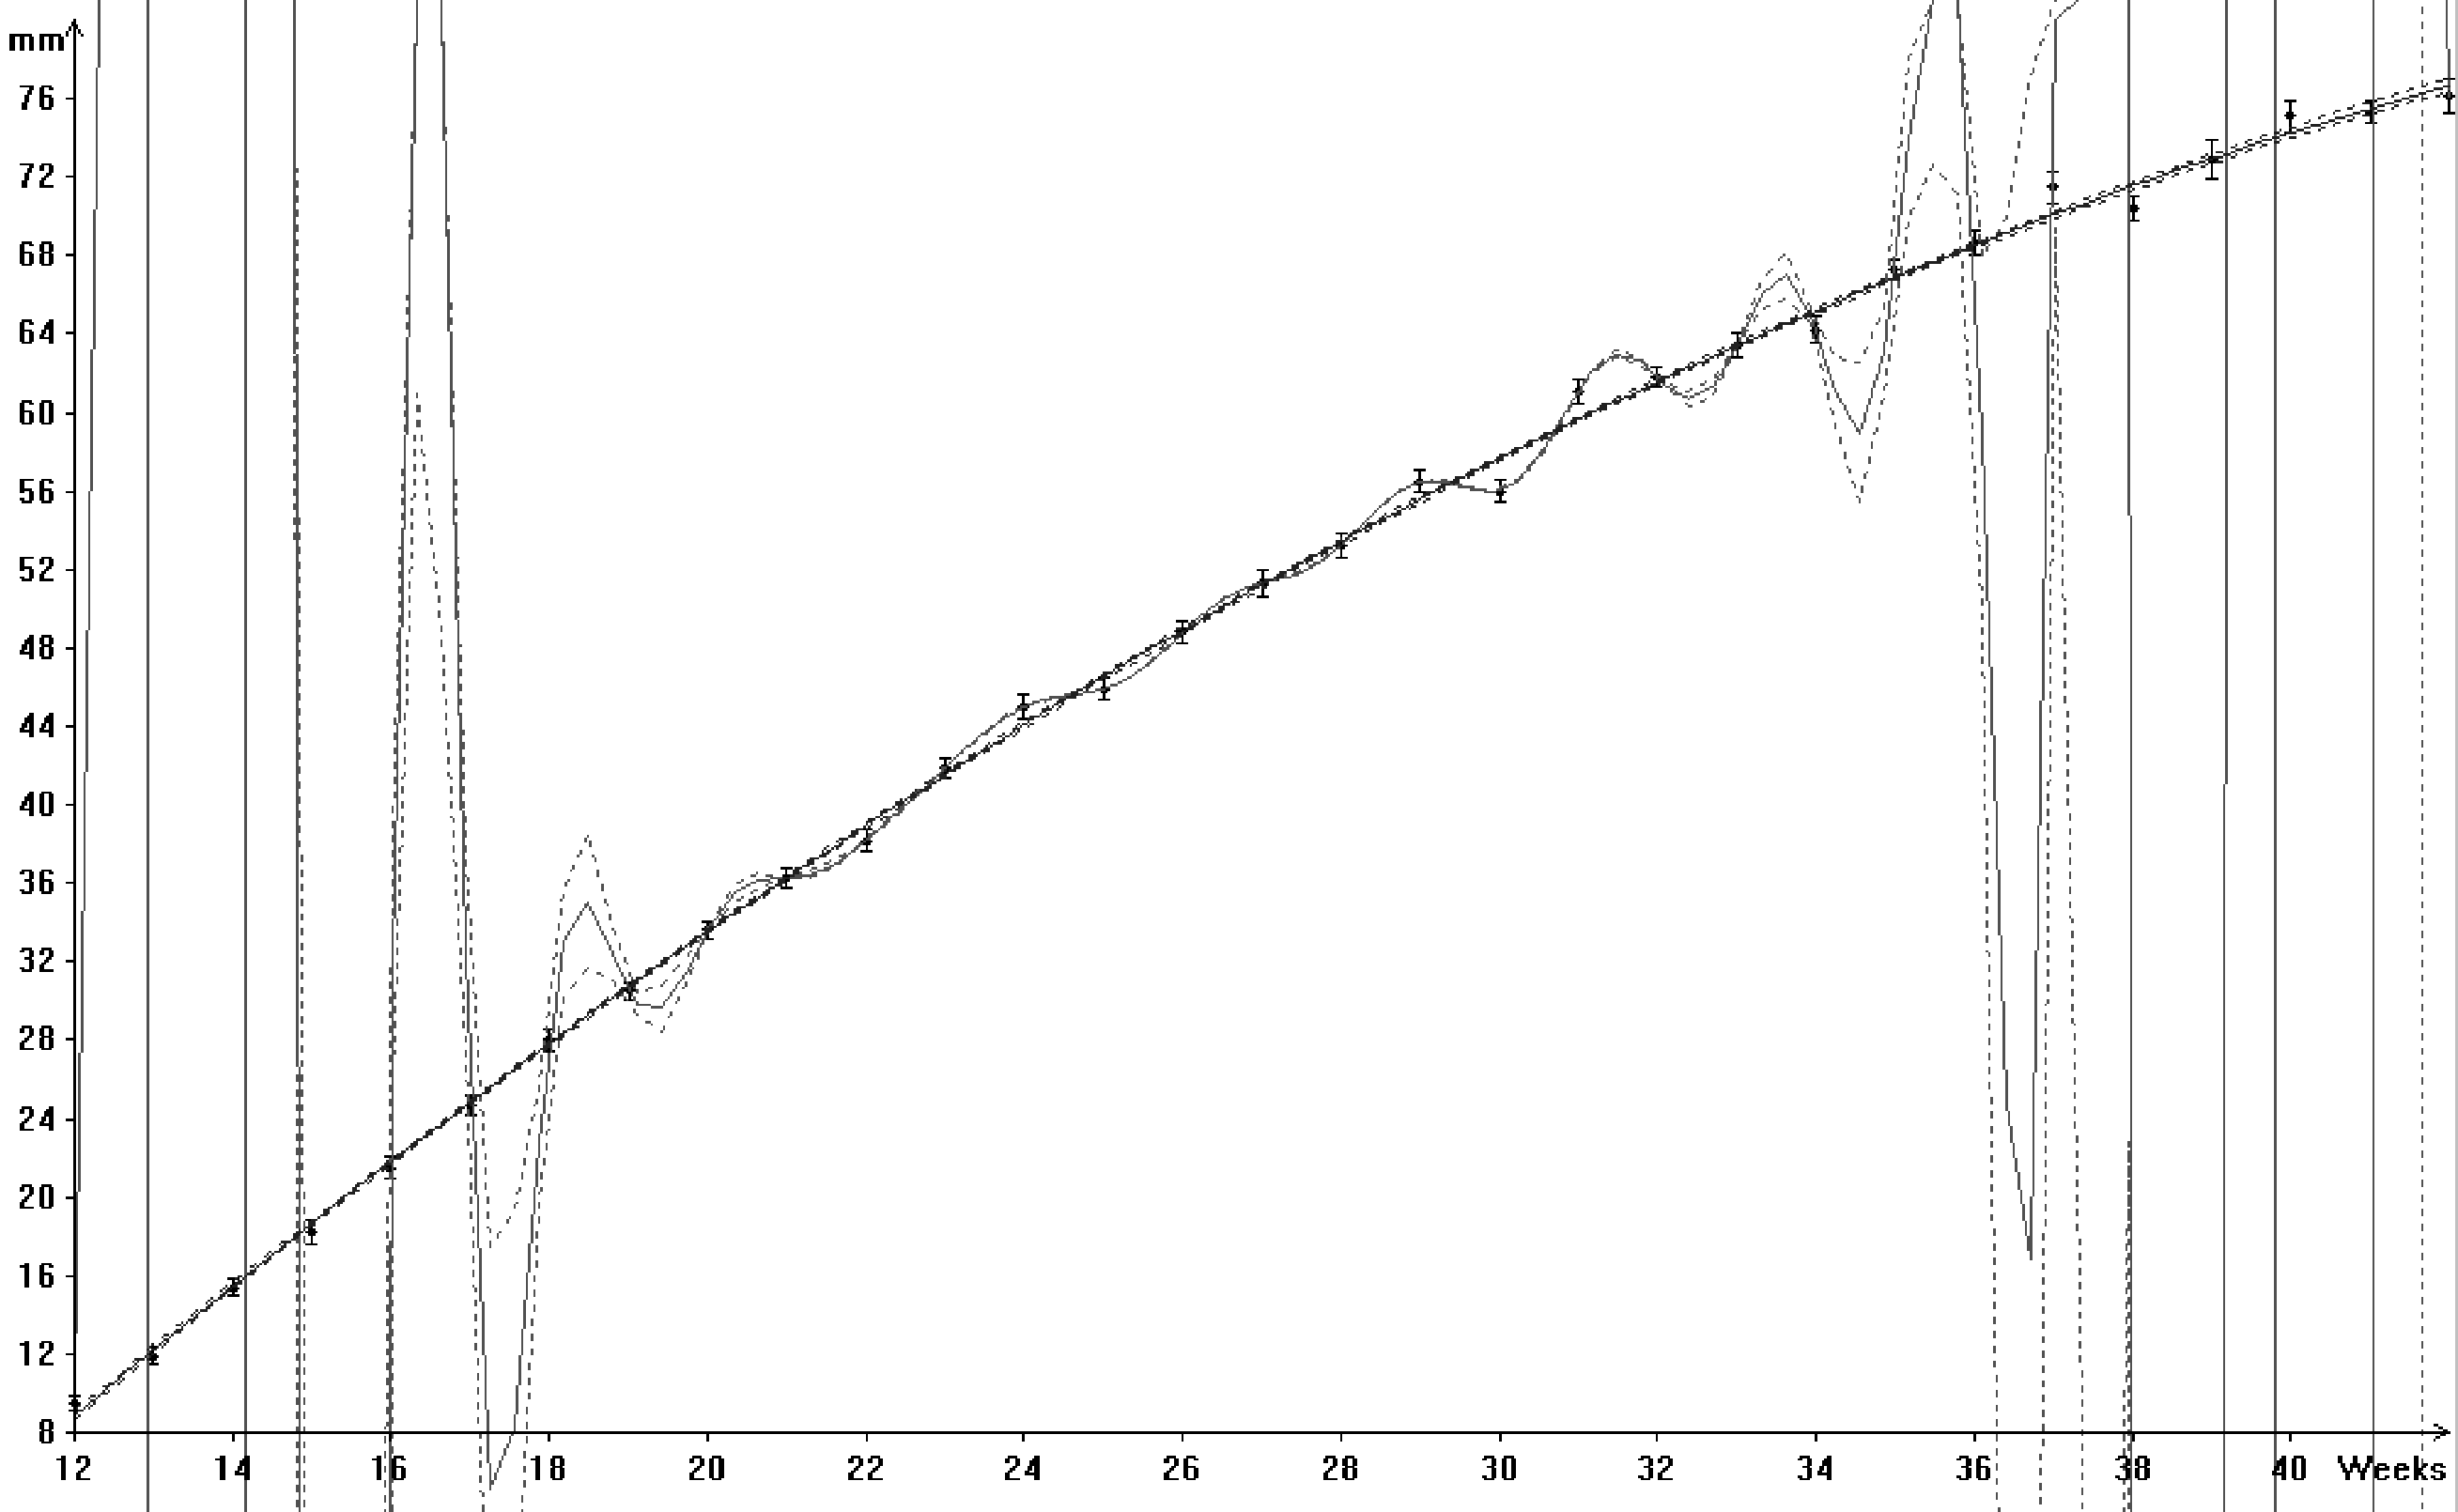
\includegraphics[width=12cm]{Figures/FemurLength}
\caption{Example of polynomial fit} \label{fig:femurLength}
\end{figure}
Each measurement has been obtained by measuring the length of
different fetuses at the same gestational age. The measurement are
averaged and the error on the average is also calculated (\cf
section \ref{sec:moments}).

The obtained data do not follow a smooth curve since the data have
been determined experimentally. The exact date of conception
cannot be exactly determined so some fluctuation is expected, but
the major limitation of the data is to obtain an sufficient number
of measurements to smooth out the natural variations between
individuals. The data from figure \ref{fig:femurLength} have been
fitted with a second order polynomial: the result is shown with a
black thin curve. As one can see, the fit is excellent in spite of
the fluctuation of the measurements. Figure
\ref{fig:femurLengthResults} shows the fit results. This $\chi^2$
confidence level is rather good.
\begin{figure}[h]
\centering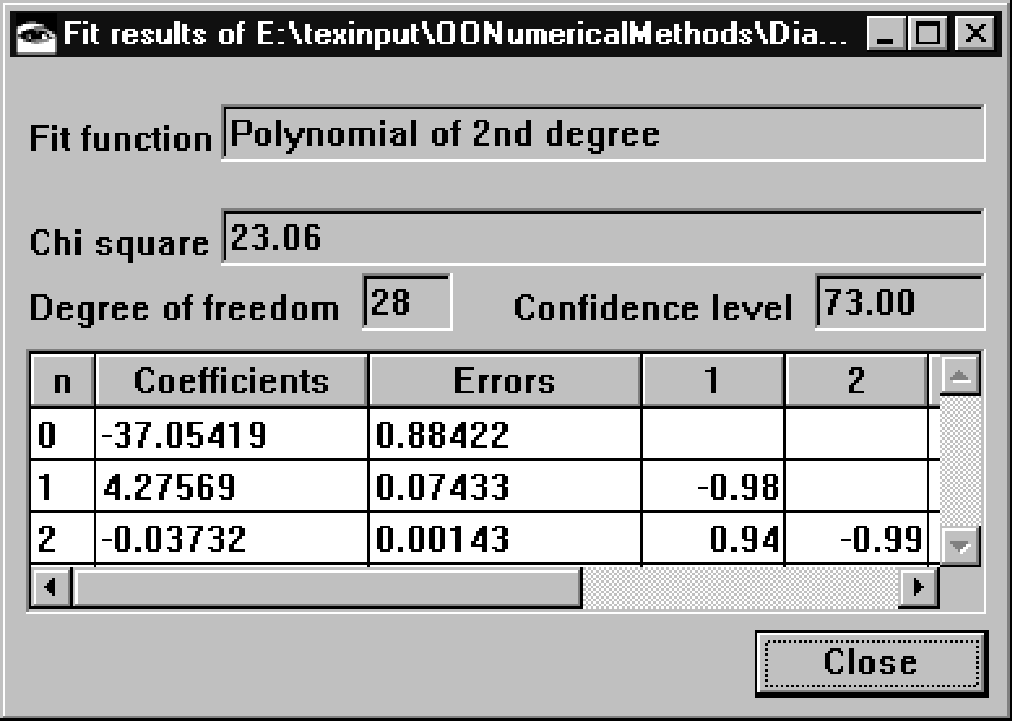
\includegraphics[width=8cm]{Figures/PolFitResults}
\caption{Fit results for the fit of figure \ref{fig:femurLength}
}\label{fig:femurLengthResults}
\end{figure}
However, the correlation coefficients are quite high. This is
usually the case with polynomial fits as each coefficient strongly
depends on the other.

The thick gray line on figure \ref{fig:femurLength} shows the
interpolation polynomial\footnote{An attentive reader will notice
that the interpolation curve dos not go through some data points.
This is an artifact of the plotting over a finite sample of points
which do not coincide with the measured data.} for comparison
(interpolation is discussed in chapter \ref{ch:interpolation}). As
the reader can see the interpolation polynomial gives unrealistic
results because of the fluctuations of the experimental data.

Polynomial fits have something in common with interpolation: a
fitted polynomial can seldom be used to extrapolate the data
outside of the interval defined by the reference points. This is
illustrated on figure \ref{fig:polFitLimit} showing a second order
polynomial fit made on a series of points. This series is
discussed in section \ref{sec:interpolgen} (figure
\ref{fig:interpolex4}).
\begin{figure}
\centering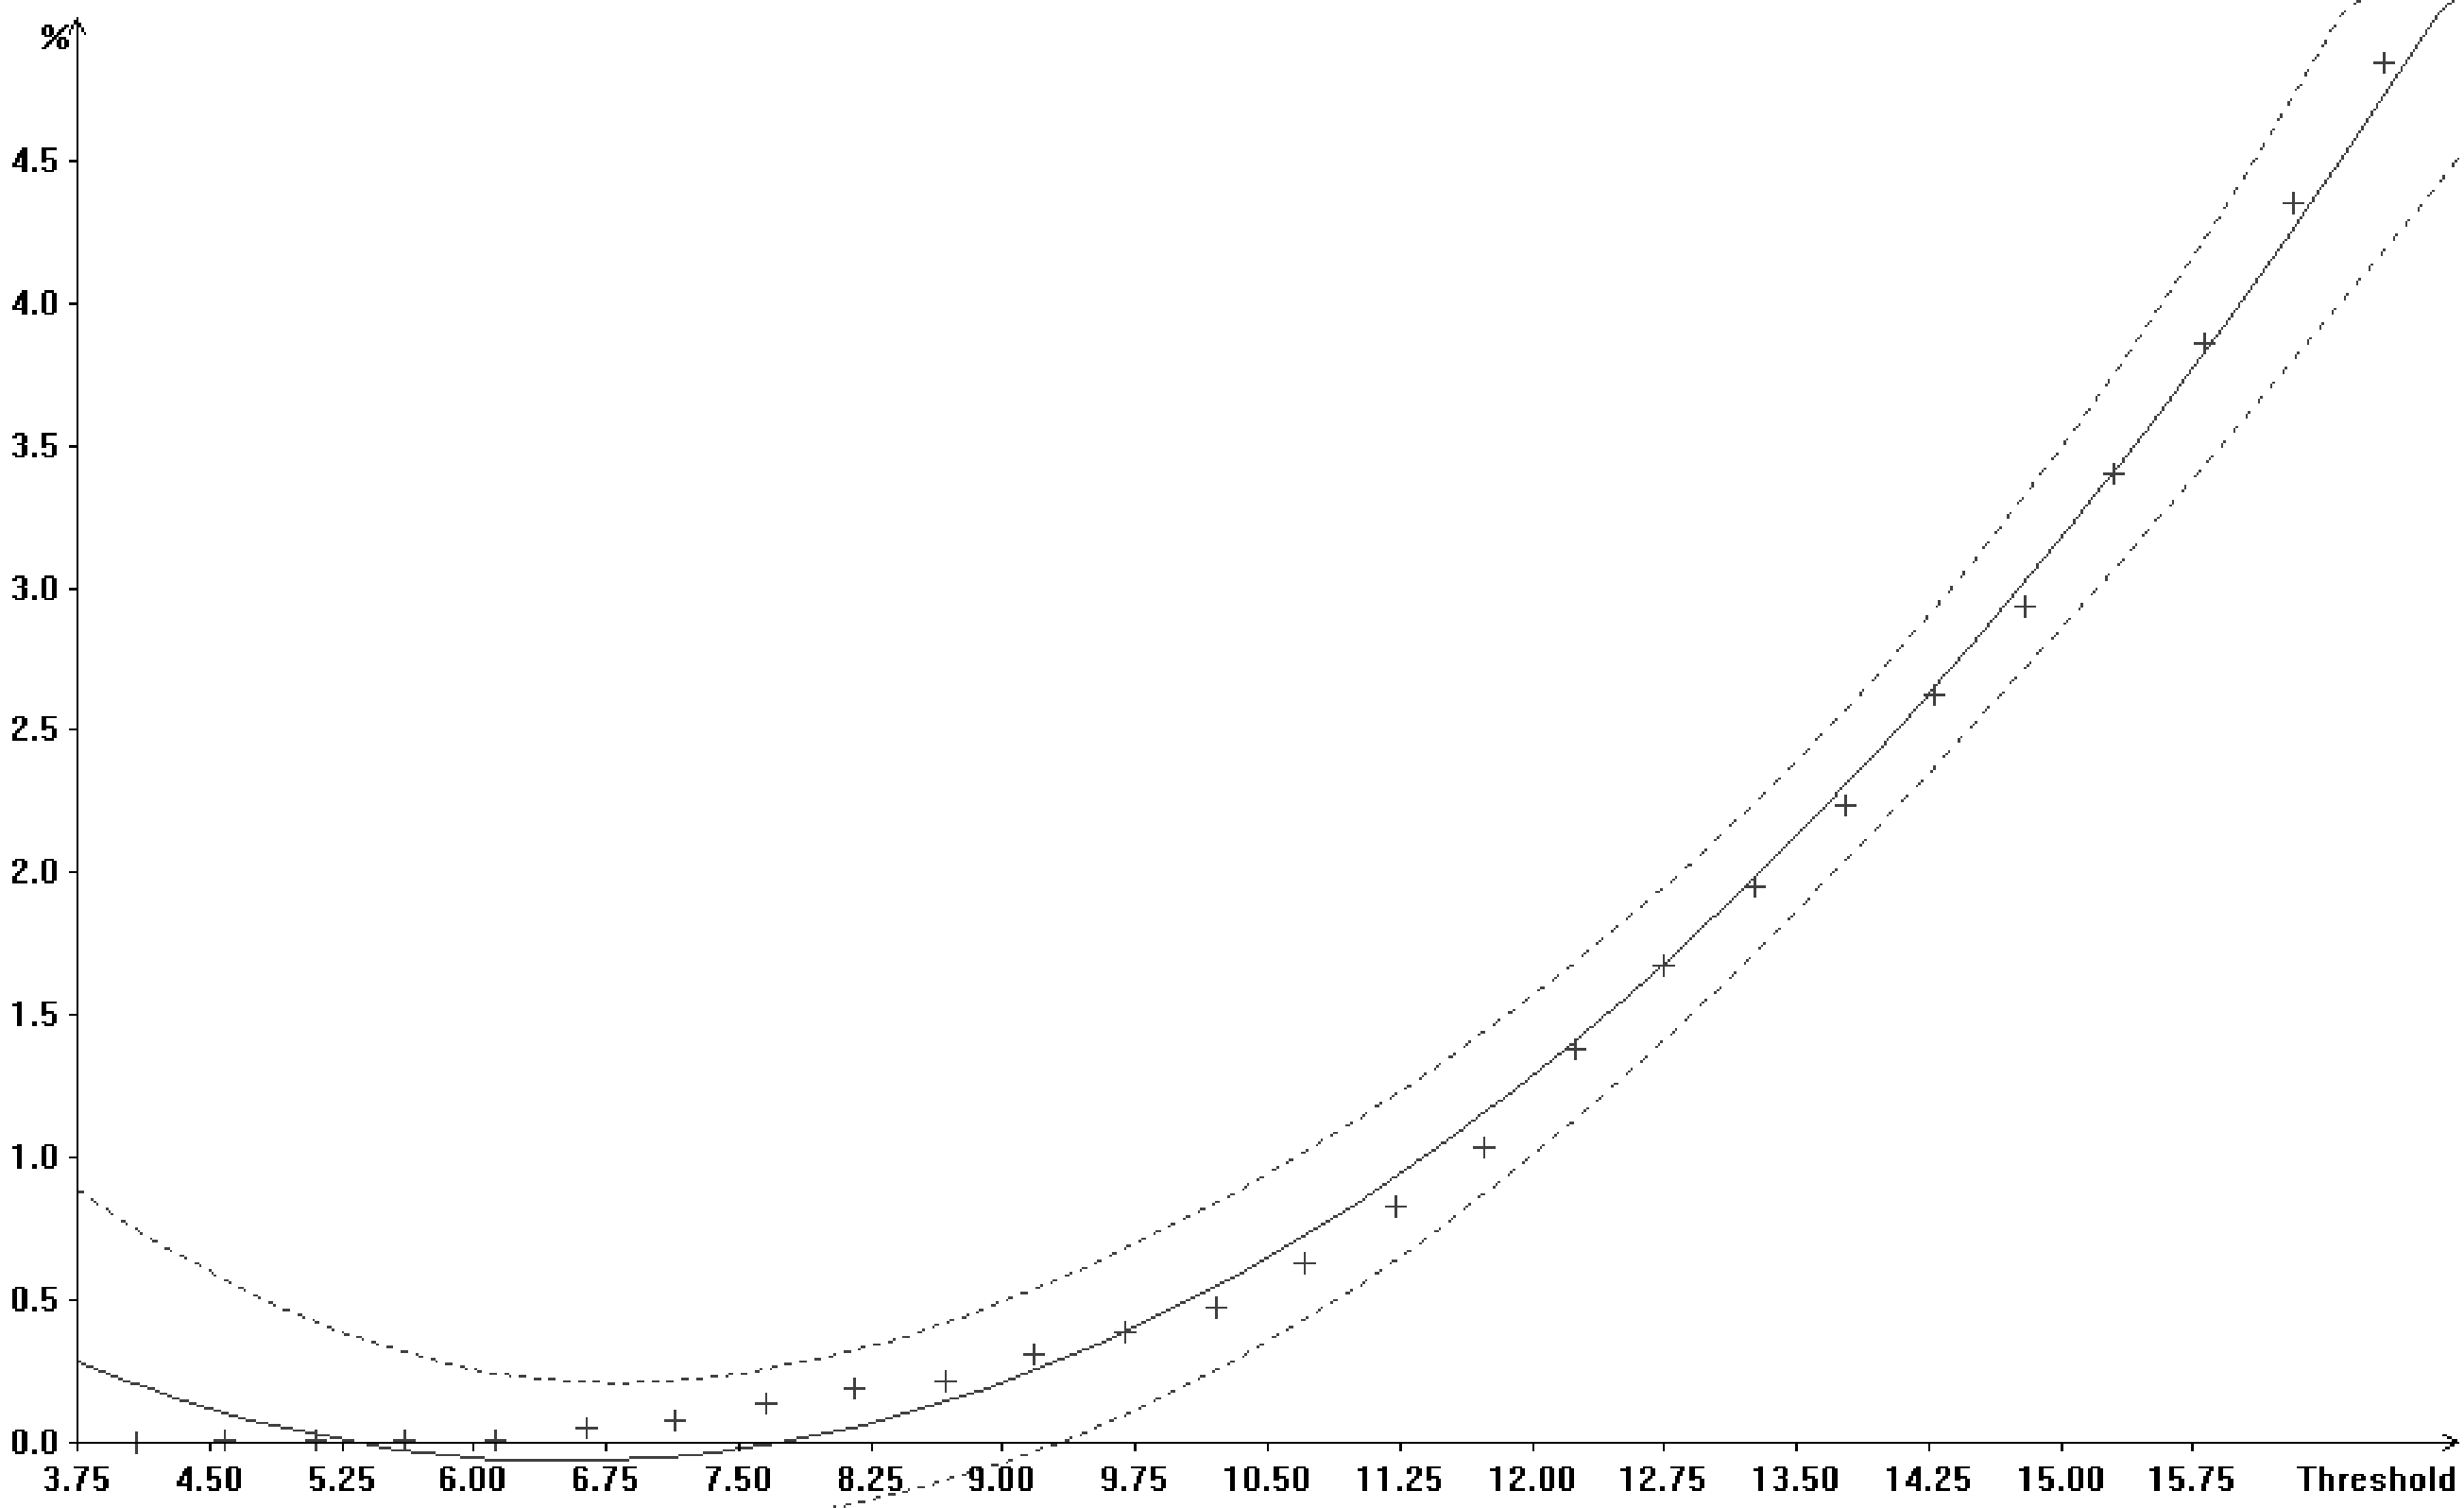
\includegraphics[width=12cm]{Figures/PolFitLimit}
\caption{Limitation of polynomial fits}\label{fig:polFitLimit}
\end{figure}
The reader can see that the fitted polynomial does not reproduce
the behavior of the data in the lower part of the region.
Nevertheless, the data are well within the estimated error. Thus,
the fit results are consistent. Unfortunately too many fit results
are presented without their estimated error. This kind of
information, however, is an essential part of a fit and should
always be deliver along with the fitted function.

This is the idea behind what we call estimated polynomials. An
estimated polynomial is a polynomial whose coefficients have been
determined by a least square fit. An estimated polynomial keeps
the error matrix of the fit is along with the coefficients of the
fitted polynomial.

\subsection{Polynomial least square fits --- Smalltalk  implementation}
\marginpar{Figure \ref{fig:estimationclasses} with the boxes {\textbf
PolynomialLeastSquareFit} and {\textbf EstimatedPolynomial} grayed.}
\label{sec:slsfpol} Listing \ref{ls:lspolynom} shows the complete
implementation in Smalltalk. The following code example show how
to perform the fit made in figure \ref{fig:femurLength}.
\begin{displaycode}{Smalltalk}
 | fit valueStream dataHolder estimation value error|
\end{displaycode}
 \hfil {\texttt<\textsl Accumulation of data into \texttt dataHolder>}
\begin{displaycode}{Smalltalk}
 fit := PMPolynomialLeastSquareFit new: 2.
 dataHolder pointsAndErrorsDo: [ :each | fit add: each].
 estimation := fit evaluate.
 value := estimation value: 20.5.
 error := estimation error: 20.5.
\end{displaycode}

The data are accumulated into a object called {\texttt dataHolder}
implementing the iterator method {\texttt pointsAndErrorsDo}. The
argument of the block used by this method is an instance of class
{\texttt PMWeightedPoint} described in section
\ref{sec:weightedPoint}. The iterator method acts on all
experimental data stored in {\texttt dataHolder}. Next, an instance of
class {\texttt PMPolynomialLeastSquareFit} is created. The argument
of the method is the degree of the polynomial; here a second order
polynomial is used. After data have been accumulated into this
object, the fit is performed by sending the method {\texttt evaluate}
to the fit object. This method returns a polynomial including the
error matrix. The last three lines compute the predicted femur
length and its error in the middle of the $20\th$ week of
pregnancy.

The Smalltalk implementation assumes the points are stored in an
object implementing the iterator method {\texttt do:}.
Any instance of
{\texttt Collection} of its subclasses will work. Each element of the
collection must be an array containing the values $x_i$, $y_i$ and
$1/\sigma_i$.
The class {\texttt PMPolynomialLeastSquareFit} keeps
this collection in the instance variable {\texttt pointCollection}. A
second instance variable, {\texttt degreePlusOne}, keeps the number of
coefficients to be estimated by the fit.

The class creation method {\texttt new:} is used to create an instance
by supplying the degree of the fit polynomial as argument. {\texttt
pointCollection} is set to a new instance of an {\texttt
OrderedCollection}. Then, new values can be added to the fit
instance with the method {\texttt add:}.

The other class creation method, {\texttt new:on:} takes two
arguments: the degree of the fit polynomial and the collection of
points. The fit result can be fetched directly after the creation.

The method {\texttt evaluate} solves equation \ref{eq:lsequs} by first
computing the inverse of the matrix ${\textbf M}$ to get the error
matrix. The coefficients are then obtained from the multiplication
of the constant vector by the error matrix.
\begin{listing} Smalltalk implementation of a polynomial least square fit \label{ls:lspolynom}
$$\halign{ #\hfil&\quad#\hfil\cr {\sl Class}& {\Large\bf DhbPolynomialLeastSquareFit}\cr
{\sl Subclass of }&{\tt Object}\cr\noalign{\vskip 1ex}

{\sl Instance variable names:}&\parbox[t]{4 in}{\tt  pointCollection degreePlusOne }\cr\noalign{\vskip 1ex}}$$


Class methods
{\parskip 1ex\par\noindent}
{\bf new:} {\tt anInteger}
\begin{verbatim}
    ^ super new initialize: anInteger
\end{verbatim}
{\bf new:} {\tt anInteger} {\bf on:} {\tt aCollectionOfPoints}
\begin{verbatim}
    ^ super new initialize: anInteger on: aCollectionOfPoints
\end{verbatim}

Instance methods
{\parskip 1ex\par\noindent}
{\bf accumulate:} {\tt aWeightedPoint} {\bf into:} {\tt aVectorOfVectors} {\bf and:} {\tt aVector}
\begin{verbatim}
OfVectors and: aVector
    | t p powers |
    p := 1.0.
    powers := aVector collect: [ :each | t := p. p := p * 
                                            aWeightedPoint xValue. t].
    aVector accumulate: powers * (aWeightedPoint yValue * 
                                               aWeightedPoint weight).
    1 to: aVector size do:
        [ :k |
          (aVectorOfVectors at: k) accumulate: powers * ((powers 
                                      at: k) * aWeightedPoint weight).
        ].
\end{verbatim}
{\bf add:} {\tt aWeightedPoint}
\begin{verbatim}
    ^ pointCollection add: aWeightedPoint
\end{verbatim}
{\bf computeEquations}
\begin{verbatim}
    | rows vector |
    vector := ( DhbVector new: degreePlusOne) atAllPut: 0 ; yourself.
    rows := ( 1 to: degreePlusOne) collect: [ :k | ( DhbVector new: 
                               degreePlusOne) atAllPut: 0 ; yourself].
    pointCollection do:
        [ :each | self accumulate: each into: rows and: vector].
    ^ Array with: ( DhbSymmetricMatrix rows: rows) with: vector
\end{verbatim}
{\bf evaluate}
\begin{verbatim}
    | system errorMatrix |
    system := self computeEquations.
    errorMatrix := ( system at: 1) inverse.
    ^ (DhbEstimatedPolynomial coefficients: errorMatrix * (system at: 
                                                                   2))
            errorMatrix: errorMatrix;
            yourself
\end{verbatim}
{\bf initialize:} {\tt anInteger}
\begin{verbatim}
    ^ self initialize: anInteger on: OrderedCollection new
\end{verbatim}
{\bf initialize:} {\tt anInteger} {\bf on:} {\tt aCollectionOfPoints}
\begin{verbatim}
    pointCollection := aCollectionOfPoints.
    degreePlusOne := anInteger + 1.
    ^ self
\end{verbatim}


\end{listing}

Listing \ref{ls:estpolynom} show the implementation of the class
{\texttt PMEstimatedPolynomial} which is a subclass of the class {\texttt PMPolynomial} containing the error matrix of the fit performed to
make a estimation of the polynomial's coefficients. The method
{\texttt error:} returns the estimated error of its value based on the
error matrix of the fit using equation \ref{eq:fitError}. The
convenience method {\texttt valueAndError:} returns an array
containing the estimated value and its error in single method
call. This is suitable for plotting the resulting curve.

\begin{listing} Smalltalk implementation of a polynomial with error \label{ls:estpolynom}
$$\halign{ #\hfil&\quad#\hfil\cr {\sl Class}& {\Large\bf DhbEstimatedPolynomial}\cr
{\sl Subclass of }&{\tt DhbPolynomial}\cr\noalign{\vskip 1ex}

{\sl Instance variable names:}&\parbox[t]{4 in}{\tt  errorMatrix }\cr\noalign{\vskip 1ex}}$$


Instance methods
{\parskip 1ex\par\noindent}
{\bf error:} {\tt aNumber}
\begin{verbatim}
    | errorVector term nextTerm |
    nextTerm := 1.
    errorVector := (coefficients collect: [ :each | term := 
            nextTerm. nextTerm := aNumber * nextTerm. term]) asVector.
    ^ (errorVector * errorMatrix * errorVector) sqrt
\end{verbatim}
{\bf errorMatrix}
\begin{verbatim}
    ^ errorMatrix
\end{verbatim}
{\bf errorMatrix:} {\tt aMatrix}
\begin{verbatim}
    errorMatrix := aMatrix.
\end{verbatim}
{\bf valueAndError:} {\tt aNumber}
\begin{verbatim}
    ^ Array with: ( self value: aNumber) with: ( self error: aNumber)
\end{verbatim}


\end{listing}


\section{Least square fit with non-linear dependence}
\label{sec:lsfnonlin} In the case of a non-linear function, the
fit can be reduced to a linear fit and a search by successive
approximations.

Let us assume that we have an approximate estimation ${\textbf p}_0$
of the parameters ${\textbf p}$. Let us define the vector $\Delta{\textbf
p}={\textbf p}-{\textbf p}_0$. One redefines the function $F\left({\textbf
x},{\textbf p}\right)$ as:
\begin{equation}
\label{eq:linexpans}
  F\left({\textbf x},{\textbf p}\right)=F\left({\textbf x},{\textbf p}_0\right)
  +\left.{\displaystyle\partial F\left({\textbf x},{\textbf
  p}\right)\over\displaystyle\partial{\textbf p}}\right|_{{\textbf p}={\textbf
  p}_0}\cdot \Delta{\textbf p}.
\end{equation}
Equation \ref{eq:linexpans} is a linear expansion\footnote{That
is, the first couples of terms of a Taylor expansion of the
function $F\left({\textbf x},{\textbf p}\right)$ around the vector ${\textbf
p}_0$ in an $m$ dimensional space.} of the function $F\left({\textbf
x},{\textbf p}\right)$ around the vector ${\textbf p}_0$ respective to the
vector ${\textbf p}$.
In equation \ref{eq:linexpans}
$\left.{\displaystyle\partial F\left({\textbf x},{\textbf
p}\right)\over\displaystyle\partial{\textbf p}}\right|_{{\textbf p}={\textbf
p}_0}$ is the gradient of the function $F\left({\textbf x},{\textbf
p}\right)$relative to the vector ${\textbf p}$ evaluated for ${\textbf
p}={\textbf p}_0$; this is a vector with the same dimension as the
vector ${\textbf p}$.
Then, one minimizes the expression in equation
\ref{eq:lsestim} respective to the vector $\Delta{\textbf p}$. This is
of course a linear problem as described in section
\ref{eq:lslinear}. Equation \ref{eq:lsmequs} becomes:
\begin{equation}
\label{eq:lslinequs}
  {\textbf M}\cdot\Delta{\textbf p}={\textbf c},
\end{equation}
where the components of the matrix ${\textbf M}$ are now defined by:
\begin{equation}
\label{eq:lsmatrix}
  M_{jk}=\sum_{i=1}^N {\displaystyle
  1\over\displaystyle\sigma_i^2}\cdot\left.{\displaystyle\partial F\left({\textbf x}_i,{\textbf
p}\right)\over\displaystyle\partial p_j}\right|_{{\textbf p}={\textbf
p}_0}\cdot\left.{\displaystyle\partial F\left({\textbf x}_i,{\textbf
p}\right)\over\displaystyle\partial p_k}\right|_{{\textbf p}={\textbf
p}_0}
\end{equation}
and the components of the vector ${\textbf c}$ are defined by:
\begin{equation}
\label{eq:lsvector}
  c_j=\sum_{i=1}^N {\displaystyle
  y_i-F\left({\textbf x}_i,{\textbf
p}_0\right)\over\displaystyle\sigma_i^2}\cdot\left.{\displaystyle\partial
F\left({\textbf x}_i,{\textbf p}\right)\over\displaystyle\partial
p_j}\right|_{{\textbf p}={\textbf p}_0}.
\end{equation}
The vector $\Delta{\textbf p}$ is obtained by solving equation
\ref{eq:lslinequs} using the algorithms described in sections
\ref{sec:lineqs} and \ref{sec:lup}. Then, we can use the vector
${\textbf p}_0+\Delta{\textbf p}$ as the new estimate and repeat the whole
process. One can show\footnote{A mathematically oriented reader
can see that this is a generalization of the Newton zero-finding
algorithm (\cf section \ref{sec:newton})to $m$ dimensions .} that
iterating this process converges toward the vector $\bar{\textbf p}$
minimizing the function $S\left({\textbf p}\right)$ introduced in
equation \ref{eq:lsestim}.

As explained in section \ref{eq:lslinear}, the inverse of the
matrix ${\textbf M}$ is the error matrix containing the variance of
each parameter and their correlation. The expression for the
estimated variance on the function $F\left({\textbf x},{\textbf p}\right)$
becomes:
\begin{equation}
\label{eq:nllserror}
  \var\left[F\left({\textbf x},{\textbf p}\right)\right]=
  \sum_{j=1}^m\sum_{k=1}^m M_{jk}^{-1}\cdot
  {\displaystyle\partial F\left({\textbf x}_i,\bar{\textbf
p}\right)\over\displaystyle\partial
p_j}\cdot{\displaystyle\partial F\left({\textbf x}_i,\bar{\textbf
p}\right)\over\displaystyle\partial p_k}.
\end{equation}
A careful examination of the error matrix can tell whether or not
the fit is meaningful.

Figure \ref{fig:lsfExample} shows an example of a least square fit
performed on a histogram with a probability density function.
\begin{figure}
\centering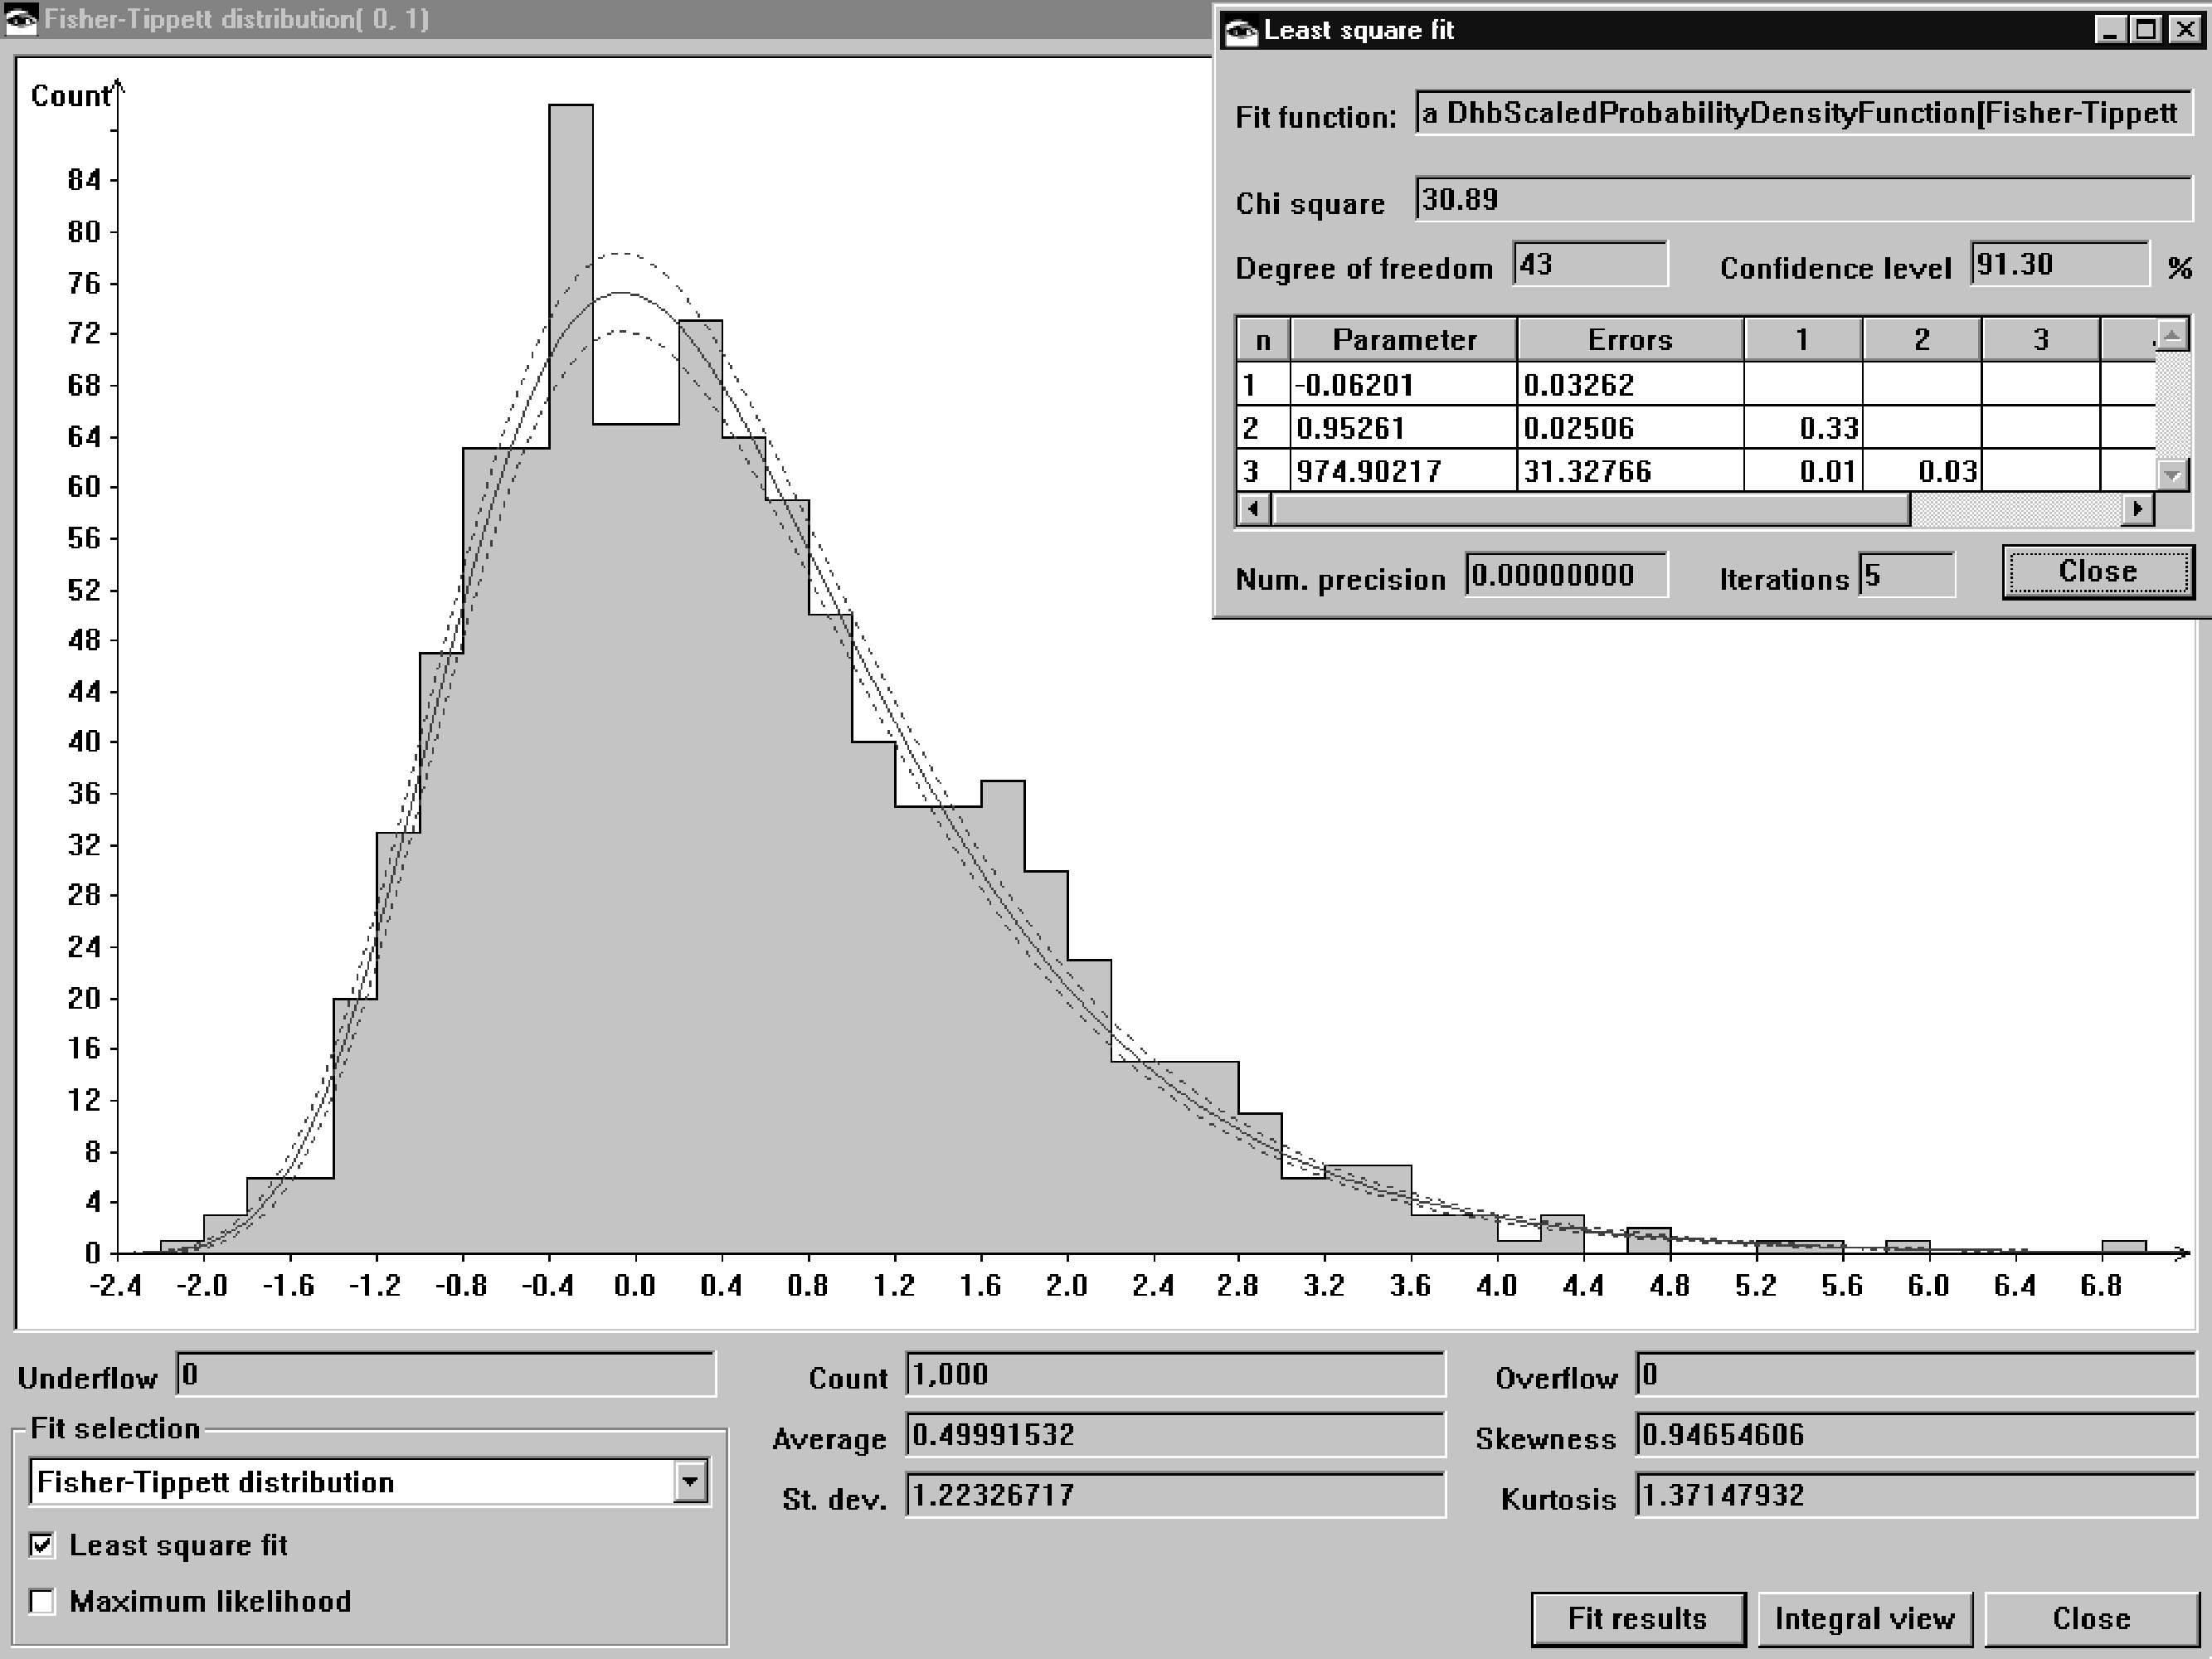
\includegraphics[width=11cm]{Figures/LeastSquareFit}
\caption{Example of a least square fit}\label{fig:lsfExample}
\end{figure}
The histogram of figure \ref{fig:lsfExample} was generated using a
random generator distributed according to a Fisher-Tippett
distribution (\cf \ref{sec:fishertippettdist}) with parameters
$\alpha = 0$ and $\beta=1$. Only 1000 events have been accumulated
into the histogram. The inset window in the upper right corner
shows the fit results. The order of the parameter are $\alpha$,
$\beta$ and the number of generated events. The solid curve laid
onto the histogram is the prediction of the fitted function; the
two dotted lines indicate the error on the prediction. The reader
can verify that the fit is excellent. The number of needed
iterations is quite low: the convergence of the algorithm is quite
good in general.

\subsection{Non-linear fit --- General implementation}
\marginpar{Figure \ref{fig:estimationclasses} with the box {\textbf
LeastSquareFit} grayed.} As we have seen the solution of a
non-linear fit can be approximated by successive approximations.
Thus, non-linear fits are implemented with a subclass of the
iterative process class described in section \ref{sec:iteration}.
Data points must be kept in a structure maintained by the object
implementing linear least square fit to be readily available at
each iteration. Thus, the data point are kept in an instance
variable.

The result of the iterative process are the parameters. Our
implementation assumes that the supplied function contains and
maintains its parameter. Thus, the instance variable corresponding
to the result of the iterative process is the fit function itself.
The parameters determined by the fit --- the result proper --- are
kept within the object implementing the supplied function. In
particular the determination of the initial values for the
iterative process are the responsibility of the fit function.
Thus, the method {\texttt initializeIterations} does not do anything.

In most cases, the number of parameters in a least square fits is
relatively small. Thus, LUP decomposition --- described in section
\ref{sec:lup} --- is sufficient to solve equation
\ref{eq:lslinequs} at each iteration. Except for the last
iteration, there is no need to compute the error matrix (the
inverse of the matrix ${\textbf M}$. The components of the error
matrix can be obtained from the LUP decomposition when the
algorithm converges.

Convergence is attained when the largest of the relative variation
of the components of the vector becomes smaller than a given
value. In addition to the fact that we are dealing with floating
point numbers, the reason for using relative precision is that the
components of the vector ${\textbf p}$ usually have different ranges.

When the fit has been obetained, convenience methods allows to
retrieve the sum of equation \ref{eq:lsmlestim} ({\texttt chiSquare})
and the confidence level of the fit ({\texttt confidenceLevel}).
Another convenience method, {\texttt valueAndError} computes the
prediction of the fit and its estimated error using equation
\ref{eq:nllserror}.

\subsection{Non-linear fit --- Smalltalk implementation}
\label{sec:slsfnonlin}Listing \ref{ls:lsfnonlin} shows the
complete implementation in Smalltalk. The following code example
shows how the data of figure \ref{fig:lsfExample} were
generated\footnote{$\ldots$up to the plotting facilities. This
could be the topic of a future book.d}.
\begin{displaycode}{Smalltalk}
\label{exs:leastSquare}
 | genDistr hist fit |
 hist := PMHistogram new.
 hist freeExtent: true.
 genDistr := PMFisherTippettDistribution shape: 0 scale: 1.
 1000 timesRepeat: [ hist accumulate: genDistr random ].
 fit := PMLeastSquareFit histogram: hist
            distributionClass: DhbFisherTippettDistribution.
 fit evaluate.
\end{displaycode}
The first two lines after the declaration define an instance of
class {\texttt PMHistogram} with automatic adjustment of the limits
(\cf section \ref{sec:shistogram}).
The next line defines an
instance of a Fisher-Tippett distribution. Then, 1000 random
numbers generated according to this distribution are accumulated
into the histogram. Next, an instance if the class {\texttt
PMLeastSquareFit} is defined with the histogram for the data
points and the desired class of the probability density function.
The corresponding scaled probability is created within the method
(\cf listing \ref{ls:lsfnonlin}). the final line performs the fit
proper. After this line, the calling application can either use
the fit object or extract the fit result to make predictions with
the fitted distribution.

The class {\texttt PMLeastSquareFit} is a subclass of {\texttt
PMIterativeProcess} described in section \ref{sec:siteration}. It
has the following instance variables:
\begin{description}
  \item[\texttt dataHolder] is the object containing the experimental
  data; this object must implement the iterator method {\texttt
  pointsAndErrorsDo:}; the block supplied to the iterator method
  takes as argument an instance of the class {\texttt
  PMWeightedPoint} described in section \ref{sec:weightedPoint};
  \item[\texttt equations] contains the components of the matrix ${\textbf
  M}$;
  \item[\texttt constants] contains the components of the vector ${\textbf
  c}$;
  \item[\texttt errorMatrix] contains the LUP decomposition of the matrix ${\textbf
  M}$;
  \item[\texttt chiSquare] contains the sum of equation \ref{eq:lsmlestim};
  \item[\texttt degreeOfFreedom] contains the degree of freedom of the
  fit.
\end{description}
The instance variables {\texttt errorMatrix}, {\texttt chiSquare} and {\texttt
degreeOfFreedom} are implemented using lazy initialization. The
method {\texttt finalizeIterations} sets the instance variables {\texttt
equations} and {\texttt constants} to {\texttt nil} to reclaim space at
the end of the fit.

The supplied fit function --- instance variable {\texttt result} ---
must implement the method {\texttt valueAndGradient:} which returns an
array containing the value of the function at the supplied
argument and the gradient vector. This is an optimization because
the gradient can be computed frequently using intermediate results
coming from the computation of the function's value.

The method {\texttt valueAndError:} is a good example of using the
vector and matrix operations described in chapter
\ref{ch:linearalgebra}.

\begin{listing} Smalltalk implementation of a non-linear
least square fit \label{ls:lsfnonlin}
$$\halign{ #\hfil&\quad#\hfil\cr {\sl Class}& {\Large\bf DhbLeastSquareFit}\cr
{\sl Subclass of }&{\tt DhbIterativeProcess}\cr\noalign{\vskip 1ex}

{\sl Instance variable names:}&\parbox[t]{4 in}{\tt  dataHolder errorMatrix chiSquare equations constants degreeOfFreedom }\cr\noalign{\vskip 1ex}}$$


Class methods
{\parskip 1ex\par\noindent}
{\bf histogram:} {\tt aHistogram} {\bf distributionClass:} {\tt aProbabilityDensityFunctionClass}
\begin{verbatim}
    ^ self points: aHistogram
        function: (DhbScaledProbabilityDensityFunction histogram: 
                                                            aHistogram
                distributionClass: aProbabilityDensityFunctionClass)
\end{verbatim}
{\bf points:} {\tt aDataHolder} {\bf function:} {\tt aParametricFunction}
\begin{verbatim}
    ^ aParametricFunction ifNotNil: [ :dp | super new initialize: 
                                                 aDataHolder data: dp]
\end{verbatim}

Instance methods
{\parskip 1ex\par\noindent}
{\bf accumulate:} {\tt aWeightedPoint}
\begin{verbatim}
    | f g |
    f := result valueAndGradient: aWeightedPoint xValue.
    g := f last.
    f := f first.
    constants accumulate: g * ((aWeightedPoint yValue - f) * 
                                               aWeightedPoint weight).
    1 to: g size do:
        [ :k |
          (equations at: k) accumulate: g * ((g at: k) * 
                                               aWeightedPoint weight).
        ].
\end{verbatim}
{\bf accumulateEquationSystem}
\begin{verbatim}
    dataHolder pointsAndErrorsDo: [ :each | self accumulate: each].
\end{verbatim}
{\bf chiSquare}
\begin{verbatim}
    chiSquare isNil
        ifTrue: [ self computeChiSquare].
    ^ chiSquare
\end{verbatim}
{\bf computeChanges}
\begin{verbatim}
    errorMatrix := DhbLUPDecomposition direct: equations.
    ^ errorMatrix solve: constants
\end{verbatim}
{\bf computeChiSquare}
\begin{verbatim}
    chiSquare := 0.
    degreeOfFreedom := self numberOfFreeParameters negated.
    dataHolder pointsAndErrorsDo:
        [ :each |
          chiSquare := ( each chi2Contribution: result) + chiSquare.
          degreeOfFreedom := degreeOfFreedom + 1.
        ].
\end{verbatim}
{\bf computeEquationSystem}
\begin{verbatim}
    constants atAllPut: 0.
    equations do: [ :each | each atAllPut: 0].
    self accumulateEquationSystem.
\end{verbatim}
{\bf confidenceLevel}
\begin{verbatim}
    ^ (DhbChiSquareDistribution degreeOfFreedom: self 
                      degreeOfFreedom) confidenceLevel: self chiSquare
\end{verbatim}
{\bf degreeOfFreedom}
\begin{verbatim}
    degreeOfFreedom isNil
        ifTrue: [ self computeChiSquare].
    ^ degreeOfFreedom
\end{verbatim}
{\bf errorMatrix}
\begin{verbatim}
    ^ DhbSymmetricMatrix rows: errorMatrix inverseMatrixComponents
\end{verbatim}
{\bf evaluateIteration}
\begin{verbatim}
    | changes maxChange |
    self computeEquationSystem.
    changes := self computeChanges.
    result changeParametersBy: changes.
    maxChange := 0.
    result parameters with: changes do: 
        [ :r :d | maxChange := ( d / r) abs max: maxChange].
    ^maxChange
\end{verbatim}
{\bf finalizeIterations}
\begin{verbatim}
    equations := nil.
    constants := nil.
    degreeOfFreedom := nil.
    chiSquare := nil
\end{verbatim}
{\bf fitType}
\begin{verbatim}
    ^'Least square fit'
\end{verbatim}
{\bf initialize:} {\tt aDataHolder} {\bf data:} {\tt aParametricFunction}
\begin{verbatim}
    dataHolder := aDataHolder.
    result := aParametricFunction.
    ^ self
\end{verbatim}
{\bf initializeIterations}
\begin{verbatim}
    | n |
    n := self numberOfParameters.
    constants := (DhbVector new: n)
                atAllPut: 0;
                yourself.
    equations := (1 to: n) collect: 
                    [:k | 
                    (DhbVector new: n)
                        atAllPut: 0;
                        yourself]
\end{verbatim}
{\bf numberOfFreeParameters}
\begin{verbatim}
    ^ self numberOfParameters
\end{verbatim}
{\bf numberOfParameters}
\begin{verbatim}
    ^ result parameters size
\end{verbatim}
{\bf value:} {\tt aNumber}
\begin{verbatim}
    ^ result value: aNumber
\end{verbatim}
{\bf valueAndError:} {\tt aNumber}
\begin{verbatim}
    | valueGradient |
    valueGradient := result valueAndGradient: aNumber.
    ^Array with: valueGradient first
           with: ( valueGradient last * ( self errorMatrix * 
                                             valueGradient last)) sqrt
\end{verbatim}


\end{listing}

\section{Maximum likelihood fit of a probability density function}
\label{sec:mlfhist} In section \ref{sec:histogram} histograms have
been discussed as a way to represent a probability density
function directly from experimental data. In this section we shall
show that the maximum likelihood estimation can easily be applied
to the data gathered in a histogram in order to determine the
parameters of a hypothesized probability density function.

In general the maximum likelihood fit of a probability density
function to a histogram is much faster than the corresponding
least square fit because the number of free parameters is lower,
as we shall see in this section. In addition, the maximum
likelihood estimation is unbiased and is therefore a better
estimation than the least square fit estimation, especially when
the histogram is sparsely populated. Thus, a maximum likelihood
fit is the preferred way of finding the parameters of a
probability density function from experimental data collected in a
histogram.

Let $m$ be the number of bins in the histogram and let $n_i$ be
the content of the $i^{\mathop{\textrm th}}$ bin. Let $P_i\left({\textbf
p}\right)$ the probability of observing a value in the
$i^{\mathop{\textrm th}}$ bin. The likelihood function $L\left({\textbf
p}\right)$ is the probability of observing the particular
histogram. Since the hypothesis of a probability density function
does not constrain the total number of values collected into the
histogram, the total number of collected values can be considered
as constant. As a consequence, a maximum likelihood fit has one
parameter less than a least square fit using the same function.
Since the total number is unconstrained, the probability of
observing the particular histogram is given by a multinomial
probability. Thus, the likelihood function can be written as:
\begin{equation}
\label{eq:mlfhist}
  L\left({\textbf p}\right)=N!\prod_{i=1}^m{\displaystyle P_i\left({\textbf
  p}\right)^{n_i}\over\displaystyle n_i!},
\end{equation}
where $N=\sum_{i=1}^m n_i$ is the total number of values collected
into the histogram. As we have seen in section \ref{sec:mlf},
finding the maximum of $L\left({\textbf p}\right)$ is equivalent of
finding the maximum of the function $I\left({\textbf p}\right)$. Since
$N$ is a constant, we use a renormalized function:
\begin{equation}
\label{eq:mlogfhist} I\left({\textbf p}\right)=\ln {\displaystyle
M\left({\textbf p}\right) \over\displaystyle N!}=\sum_{i=1}^m n_i \ln
P_i\left({\textbf p}\right).
\end{equation}
Finding the maximum of the function $I\left({\textbf p}\right)$ is
equivalent to solving the following system of non-linear
equations:
\begin{equation}
\label{eq:mlfsys} {\displaystyle\partial I\left({\textbf p}\right)
\over\displaystyle\partial{\textbf p}}=\sum_{i=1}^m {\displaystyle n_i
\over\displaystyle P_i\left({\textbf
p}\right)}\cdot{\displaystyle\partial P_i\left({\textbf p}\right)
\over\displaystyle\partial{\textbf p}}=0.
\end{equation}
This system can be solved with a search by successive
approximations, where a system of linear equations must be solved
at each step. The technique used is similar to the one described
in section \ref{sec:lsfnonlin}. In this case, however, it is more
convenient to expand the inverse of the probability density
function around a previous approximation as follows:
\begin{equation}
{\displaystyle 1\over\displaystyle P_i\left({\textbf p}\right)} =
{\displaystyle 1\over\displaystyle P_i\left({\textbf p}_0\right)} -
{\displaystyle 1\over\displaystyle P_i\left({\textbf
p}_0\right)^2}\cdot \left.{\displaystyle\partial P_i\left({\textbf
p}\right) \over\displaystyle\partial{\textbf p}}\right|_{{\textbf p}={\textbf
p}_0}\cdot\Delta{\textbf p}.
\end{equation}
This expansion can only be defined over a range where the
probability density function is not equal to zero. Therefore, this
expansion of the maximum likelihood estimation cannot be used on a
histogram where bins with non-zero count are located on a range
where the probability density function is equal to
zero\footnote{Equation \ref{eq:mlogfhist} shows that the bins over
which the probability density function is zero give no
information.}. Contrary to a least square fit, bins with zero
count do not participate to the estimation.

Now equation \ref{eq:mlfsys} becomes a system of linear equations
of the type:
\begin{equation}
\label{eq:mlflinequs}
  {\textbf M}\cdot\Delta{\textbf p}={\textbf c},
\end{equation}
where the components of the matrix ${\textbf M}$ are now defined by:
\begin{equation}
\label{eq:mlfmatrix}
 M_{jk}=\sum_{i=1}^m {\displaystyle
n_i\over\displaystyle P_i\left({\textbf p}_0\right)^2
}\cdot\left.{\displaystyle\partial P_i\left({\textbf p}_0\right)
\over\displaystyle\partial p_j} \right|_{{\textbf p}={\textbf
p}_0}\cdot\left.{\displaystyle\partial P_i\left({\textbf p}_0\right)
\over\displaystyle\partial p_k} \right|_{{\textbf p}={\textbf p}_0},
\end{equation}
and those of the vector ${\textbf c}$ by:
\begin{equation}
\label{eq:mlfvector}
 c_j=\sum_{i=1}^m {\displaystyle
n_i\over\displaystyle P_i\left({\textbf p}_0\right)
}\cdot\left.{\displaystyle\partial P_i\left({\textbf p}_0\right)
\over\displaystyle\partial p_j} \right|_{{\textbf p}={\textbf p}_0}.
\end{equation}

As discussed at the beginning of this section, the maximum
likelihood estimation for a histogram cannot determine the total
count in the histogram. The estimated total count, $\bar{N}$, is
estimated with the following hypothesis:
\begin{equation}
   n_i=\bar{N}P\left(\bar{\textbf p}\right),
\end{equation}
where $\bar{\textbf p}$ is the maximum likelihood estimation of the
distribution parameters. The estimation is performed using
$\bar{N}$ as the only variable. The maximum likelihood estimation
cannot be solved analytically, however, the least square
estimation can.

As we have seen in section \ref{sec:chitesthist} the variance of
the bin count is the estimated bin content. Thus, the function to
minimize becomes:
\begin{equation}
\label{eq:mlfnorm}
S\left(\bar{N}\right)=\sum_{i=1}^m{\displaystyle\left[n_i-\bar{N}
P_i\left(\bar{\textbf p}\right)\right]^2
\over\displaystyle\bar{N}P_i\left(\bar{\textbf p}\right)}
\end{equation}
The value of $\bar{N}$ minimizing the expression of equation
\ref{eq:mlfnorm} is:
\begin{equation}
\label{eq:mlfnormsol}
\bar{N}=\sqrt{{\displaystyle\sum_{i=1}^m
n_i^2 / P_i\left(\bar{\textbf p}\right) \over\displaystyle\sum_{i=1}^m
P_i\left(\bar{\textbf p}\right)}}.
\end{equation}
and the estimated error on $\bar{N}$ is given by
\begin{equation}
\label{eq:mlfnormsigma}
\sigma_{\bar{N}}=\sqrt{{\displaystyle\sum_{i=1}^m n_i^2 /
P_i\left(\bar{\textbf p}\right) \over\displaystyle 2 \bar{N}}}.
\end{equation}

After computing $\bar{N}$ using equation \ref{eq:mlfnormsol}, the
goodness of the maximum likelihood fit can be estimated by
calculating the $\chi^2$ confidence level of
$S\left(\bar{N}\right)$ given by equation \ref{eq:mlfnorm}.

Figure \ref{fig:mlfExample} shows an example of a maximum
likelihood fit performed on the same histogram as in figure
\ref{fig:lsfExample}.
\begin{figure}
\centering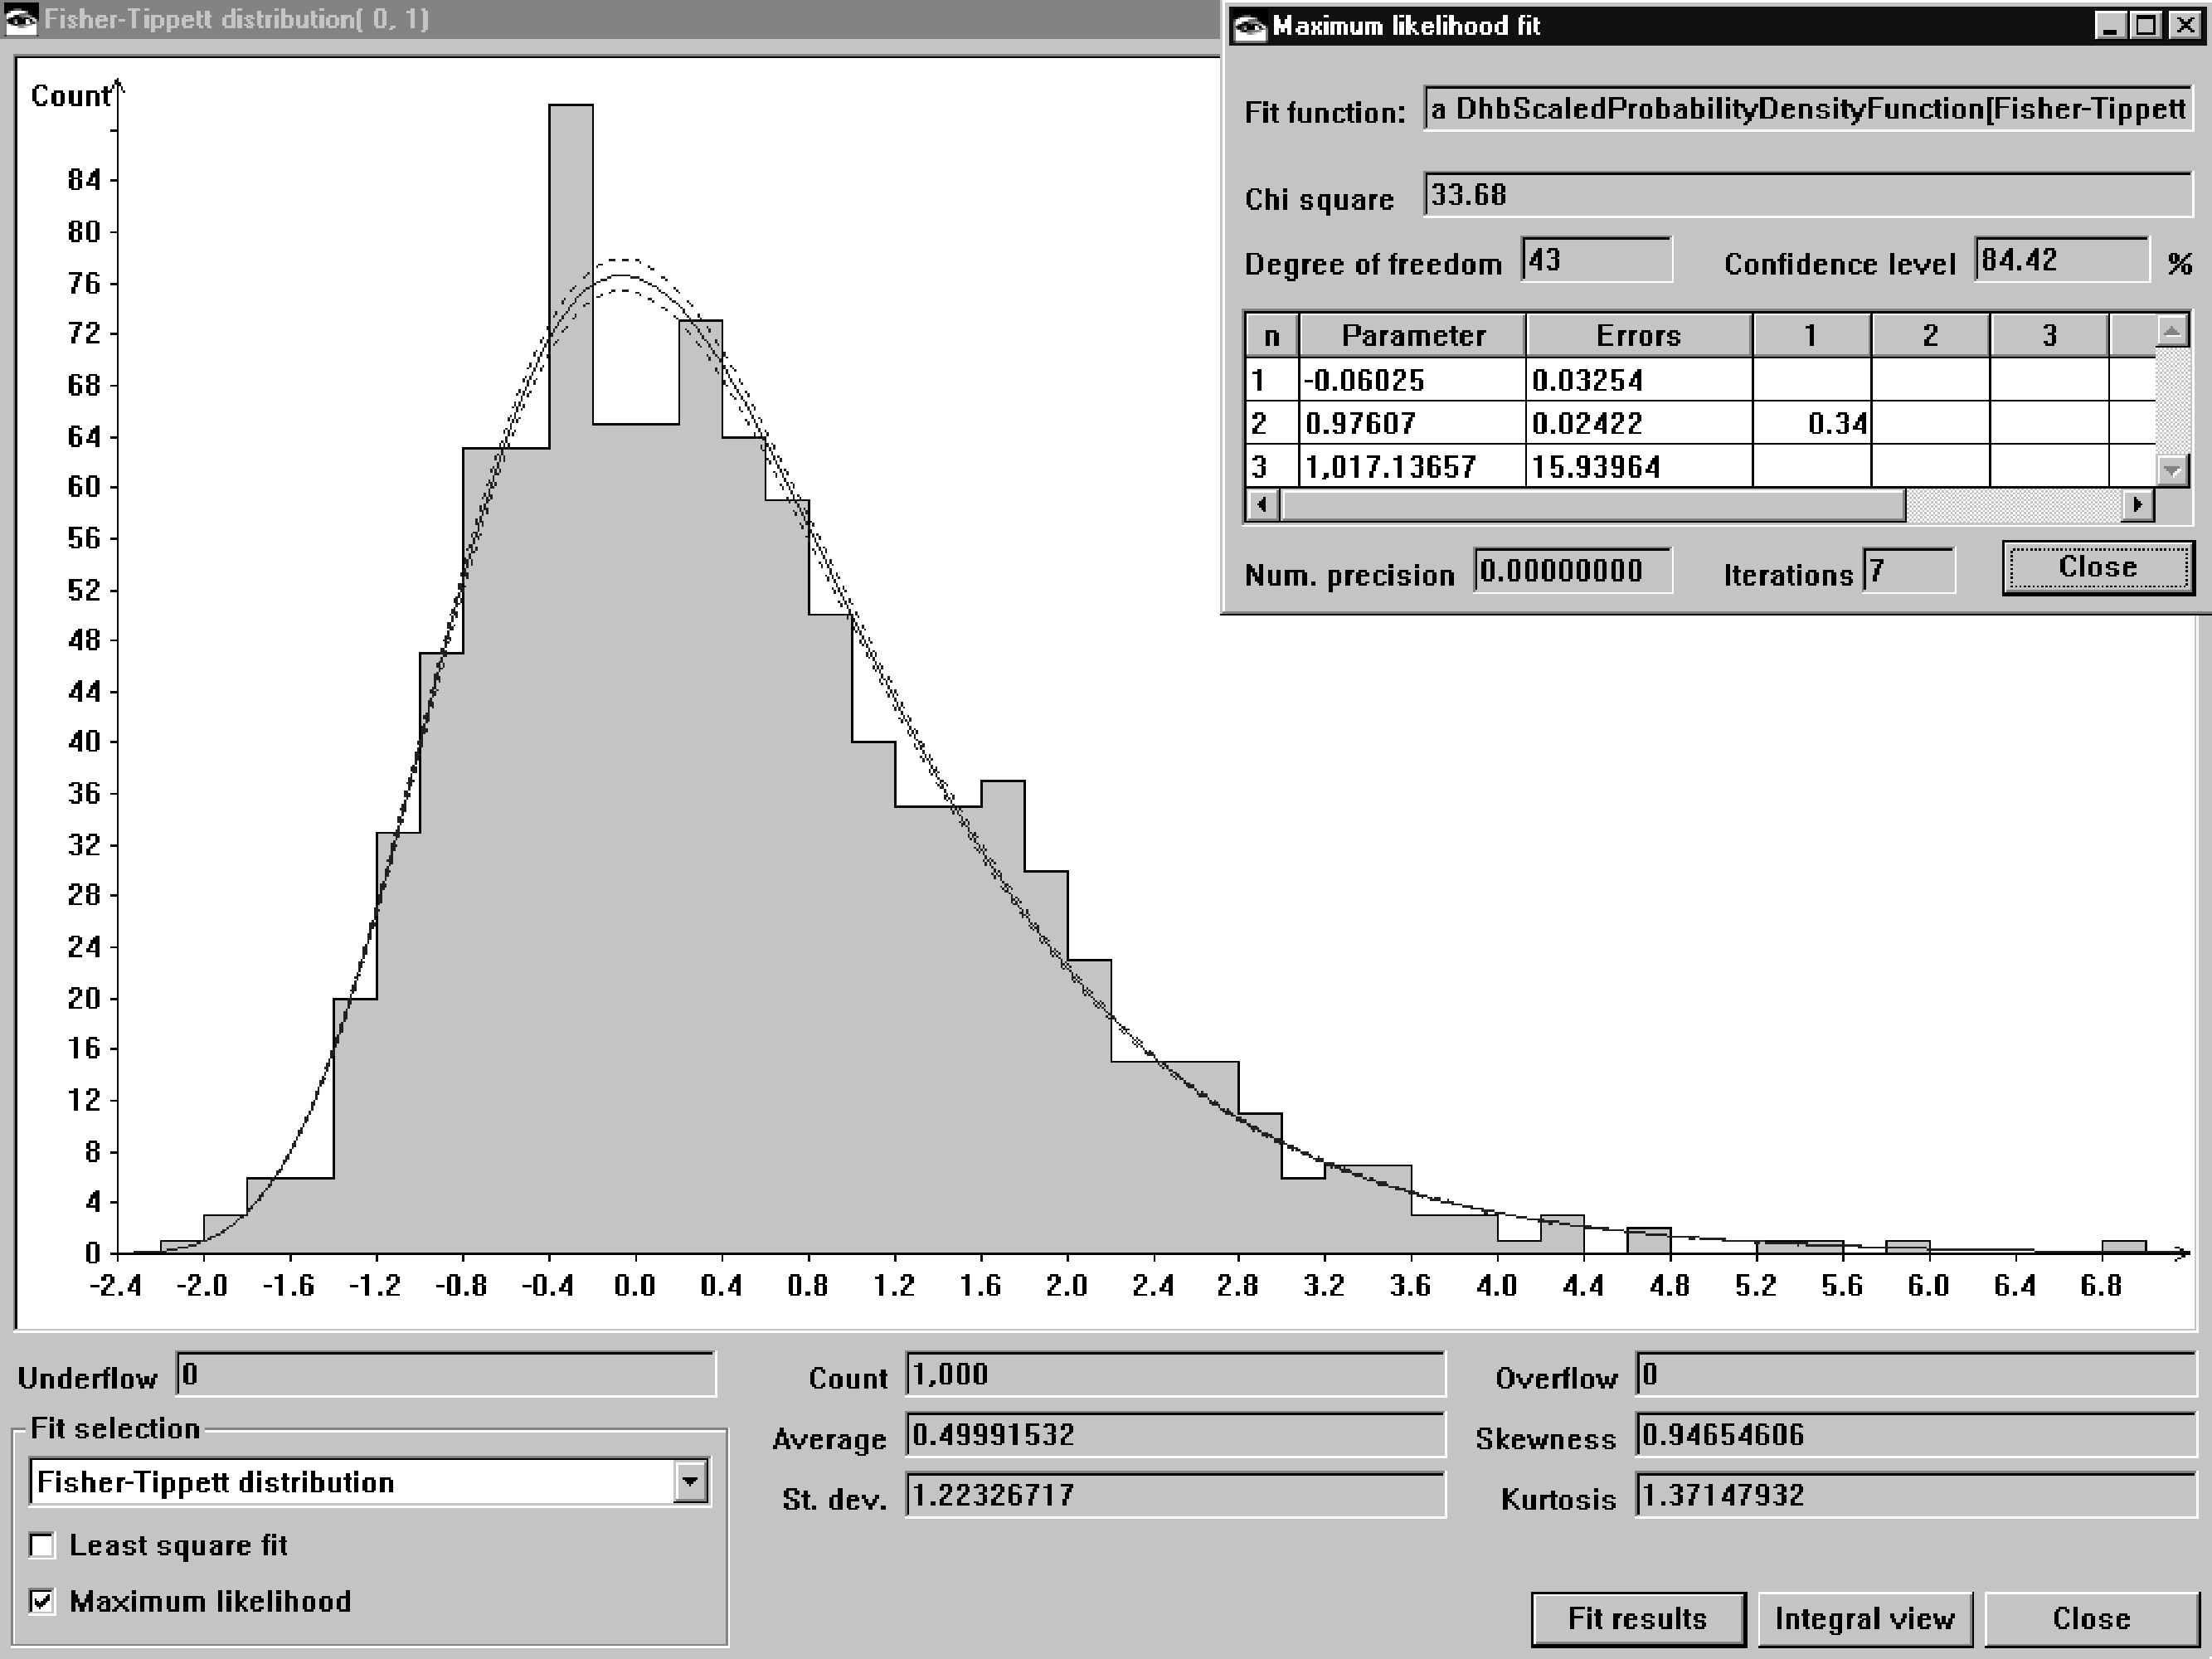
\includegraphics[width=11cm]{Figures/MaximumLikelihoodFit}
\caption{Example of a maximum likelihood
fit}\label{fig:mlfExample}
\end{figure}
The inset window in the upper right corner shows the fit resultsin
the same order as figure \ref{fig:lsfExample}. The correlation
coefficients, however, are not shown for the normalization since
it is not determined as part of the fit. The solid curve laid onto
the histogram is the prediction of the fitted function; the two
dotted lines indicate the error on the prediction. The reader can
see that the fit is as good as the least square fit. Of course,
the $\chi^2$ test is significantly higher with a correspondingly
lower confidence level. This mostly comes from the fact that a
maximum likelihood fit does not use the bins with zero count. In
fact, the reader can see that the count in the histogram
(normalization) estimated by the maximum likelihood fit is higher
than in the case of the least square fit.

\subsection{Maximum likelihood fit --- General  implementation}
\marginpar{Figure \ref{fig:estimationclasses} with the box {\textbf
MaximumLikekihoodHistogramFit} grayed.} A maximum likelihood fit
of a probability density function on a histogram is very similar
to a least square fit of a histogram with a scaled probability
distribution. There are two major differences: first the number of
parameters is lower; second the computation of the matrix and
vectors is not the same. Otherwise, most of the structure of a
least square fit can be reused.

Instead of creating special methods to compute the gradient of the
fitted function using a new set of parameters, our implementation
uses the same gradient calculation than the one used by the least
square fit. This is possible if the component of the gradient
relative to the normalization is placed at the end. Since the
computation of this component does not require additional
calculation, the additional time required by the re-using of the
gradient's computation is negligible. Since the fit function is a
scaled probability distribution the current normalization is kept
in an instance variable and the normalization of the fitted
function is set to 1 for the duration of the iterations. When the
algorithm is completed, the estimated normalization is put back
into the fit function.

The computation of the normalization (equation
\ref{eq:mlfnormsol}) and that of its error (equation
\ref{eq:mlfnormsigma}) is performed in the method {\texttt
finalizeIterations}.

\subsection{Maximum likelihood fit --- Smalltalk  implementation}
\label{sec:smlfhist}Listing \ref{ls:mlf} shows the complete
implementation in Smalltalk. The following code example shows how
figure \ref{fig:mlfExample} was generated up to the plotting
facilities.
\begin{displaycode}{Smalltalk}
 | genDistr hist fit |
 hist := PMHistogram new.
 hist freeExtent: true.
 genDistr := PMFisherTippettDistribution shape: 0 scale: 1.
 1000 timesRepeat: [ hist accumulate: genDistr random ].
 fit := PMMaximumLikekihoodHistogramFit histogram: hist
            distributionClass: PMFisherTippettDistribution.
 fit evaluate.
\end{displaycode}
As the reader can see the only difference with code example
\ref{exs:leastSquare} is the name of the class in the statement
where the instance of the fit is created.

\noindent The class {\texttt PMMaximumLikekihoodHistogramFit} is a
subclass of the class {\texttt PMLeastSquareFit}. It has the
following additional instance variables:
\begin{description}
  \item[\texttt count] the estimated normalization, that is $\bar{N}$;
  \item[\texttt countVariance] the estimated variance of $\bar{N}$.
\end{description}
The variance is kept instead of the error because the most
frequent use of this quantity is in computing the estimated error
on the predicted value. In the method {\texttt valueAndError:} this
computation requires the combination of the error of the fit ---
that is, equation \ref{eq:fitError} --- with the error on the
normalization. An accessor method is provided for the variable
{\texttt count}. The method {\texttt normalizationError} calculates the
error on the normalization.

The method {\texttt accumulate:} uses the vector operations to
calculate the terms of the sums in equations \ref{eq:mlfmatrix}
and \ref{eq:mlfvector}. Because of the lower number of parameters,
the routine {\texttt computeChanges:} places in the vector
$\Delta_{\textbf p}$ an additional zero element corresponding to the
normalization in the case of the least square fit.

The method {\texttt finalizeIterations} calculates the estimated value
of the normalization (equation \ref{eq:mlfnorm}) and its variance
(square of equation \ref{eq:mlfnormsol}). After this, it sets the
obtained normalization into the scaled probability distribution.

\begin{listing} Smalltalk implementation of a maximum likelihood fit \label{ls:mlf}
$$\halign{ #\hfil&\quad#\hfil\cr {\sl Class}& {\Large\bf DhbMaximumLikekihoodHistogramFit}\cr
{\sl Subclass of }&{\tt DhbLeastSquareFit}\cr\noalign{\vskip 1ex}

{\sl Instance variable names:}&\parbox[t]{4 in}{\tt  count countVariance }\cr\noalign{\vskip 1ex}}$$


Instance methods
{\parskip 1ex\par\noindent}
{\bf accumulate:} {\tt aWeightedPoint}
\begin{verbatim}
    | f g temp inverseProbability|
    f := result valueAndGradient: aWeightedPoint xValue.
    g := f last copyFrom: 1 to: ( f last size - 1).
    f := f first.
    f = 0 ifTrue: [ ^nil].
    inverseProbability := 1 / f.
    temp := aWeightedPoint yValue * inverseProbability.
    constants accumulate: g * temp.
    temp := temp * inverseProbability.
    1 to: g size do:
        [ :k |
          ( equations at: k) accumulate: g * ( ( g at: k) * temp).
        ].

\end{verbatim}
{\bf computeChanges}
\begin{verbatim}
    ^super computeChanges copyWith: 0

\end{verbatim}
{\bf computeNormalization}
\begin{verbatim}
    | numerator denominator temp |
    numerator := 0.
    denominator := 0.
    dataHolder pointsAndErrorsDo: 
            [:each | 
            temp := result value: each xValue.
            temp = 0 
                ifFalse: 
                    [numerator := numerator + (each yValue squared / 
                                                                temp).
                    denominator := denominator + temp]].
    count := ( numerator / denominator) sqrt.
    countVariance := numerator / ( 4 * count).

\end{verbatim}
{\bf finalizeIterations}
\begin{verbatim}
    self computeNormalization.
    result setCount: count.
    super finalizeIterations

\end{verbatim}
{\bf fitType}
\begin{verbatim}
    ^'Maximum likelihood fit'

\end{verbatim}
{\bf initializeIterations}
\begin{verbatim}
    result setCount: 1.
    count := dataHolder totalCount.
    super initializeIterations

\end{verbatim}
{\bf normalization}
\begin{verbatim}
    ^count

\end{verbatim}
{\bf normalizationError}
\begin{verbatim}
    ^countVariance sqrt

\end{verbatim}
{\bf numberOfFreeParameters}
\begin{verbatim}
    ^super numberOfParameters

\end{verbatim}
{\bf numberOfParameters}
\begin{verbatim}
    ^super numberOfParameters - 1

\end{verbatim}
{\bf valueAndError:} {\tt aNumber}
\begin{verbatim}
    | valueGradient gradient gVar |
    valueGradient := result valueAndGradient: aNumber.
    gradient := valueGradient last copyFrom: 1 to: valueGradient last 
                                                             size - 1.
    gVar := gradient * (self errorMatrix * gradient) / count.
    ^Array with: valueGradient first
        with: ((valueGradient first / count) squared * countVariance 
                                                          + gVar) sqrt

\end{verbatim}


\end{listing}


%\ifx\wholebook\relax\else\end{document}\fi
